\section{Simulation}
In this chapter several simulations, and their respective results, are presented. It will be explained how a simplified simulation framework was developed to evaluate the performance of the algorithm in real time. Then several results are presented showing the capability of the algorithm to adapt to changes in the environment and deal with other aircraft in real-time.
\par
To validate the usage of the algorithms for real-vehicles, realistic physics simulations were performed using Gazebo. The used plugin and controller are briefly explained. A simulation is analysed to evaluate the capability of the simulated multi-rotor to follow the desired trajectories.

\subsection{Real-time avoidance}
A simplified simulation was performed to validate the real time performance of the algorithms. A simplified model of a UAV was created, this model consisted of a point with a given mass to which the control inputs were applied as forces. A simple controller was developed to transform the reference acceleration, speed and position into force inputs for the model.
The Figures \ref{fig:basic00}-\ref{fig:basic14} show the results for a real time testing of the algorithms in a complex indoor environments with unexpected obstacles appearing in the map as the model follows the trajectory.


%\null\newpage
%\null\newpage

Real time avoidance was also performed using moving obstacles. For avoiding non-cooperative intruders the algorithm assumes that these intruders travel at constant speed. Once the trajectories of these intruders might be unpredictable, the safety distance that the algorithm considers for these intruders is 3 times the one considered for static obstacles and cooperative intruders. The algorithm was also empowered to be able to simulate sensor delay.
\par
Several simulations were performed to validate the capability of avoiding moving intruders. For the first test the aircraft flies through a map of known obstacles. It was possible in this simulation to manually insert moving obstacles. This moving obstacles would start in a desired position at the top of the map and they would move (at constant speed) towards the bottom of the map. These moving obstacles are represented as circles. An avoidance of an unexpected moving obstacle is shown in Figures \ref{fig:dodM1} and \ref{fig:dodM2}.

\begin{figure}[!htb]
    \centering
    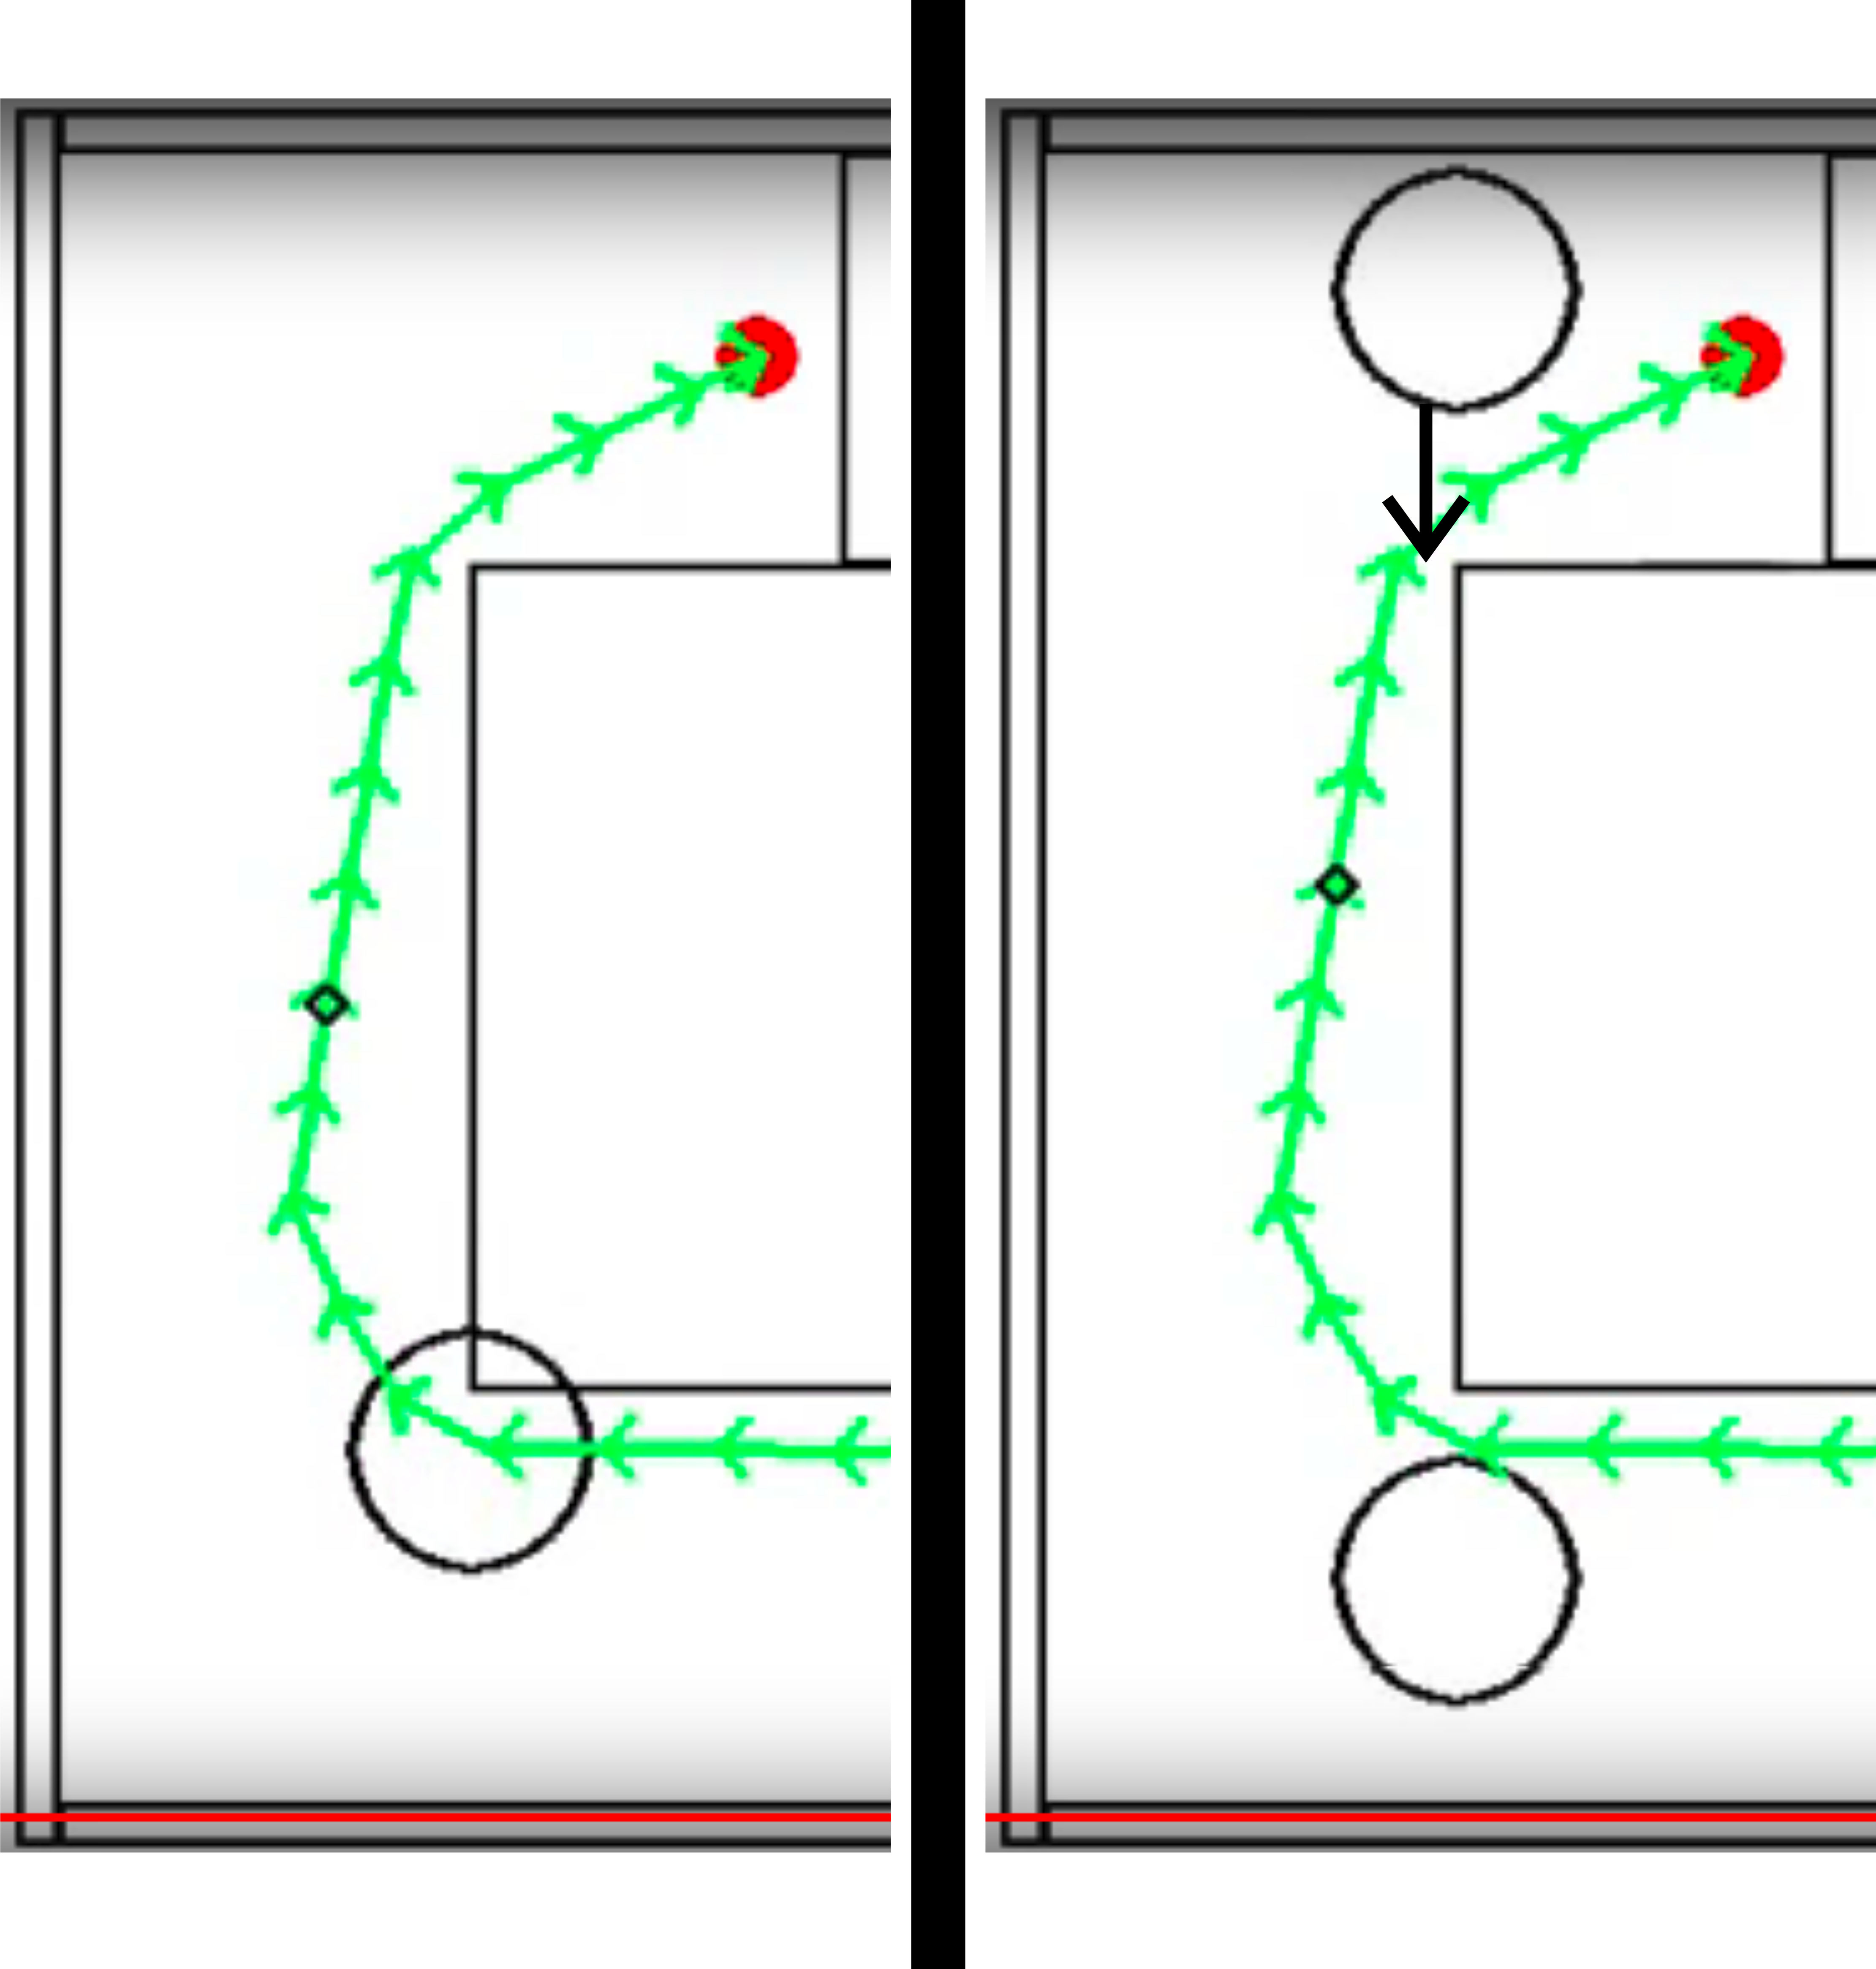
\includegraphics[width=0.5\linewidth]{Figures/07_simulation/moving/dodgeMod1.png}
    \caption{New obstacle appears, moving from the top to the bottom of the figure. (time=1m13s)}
    \label{fig:dodM1}
\end{figure}


\begin{figure}[!htb]
    \centering
    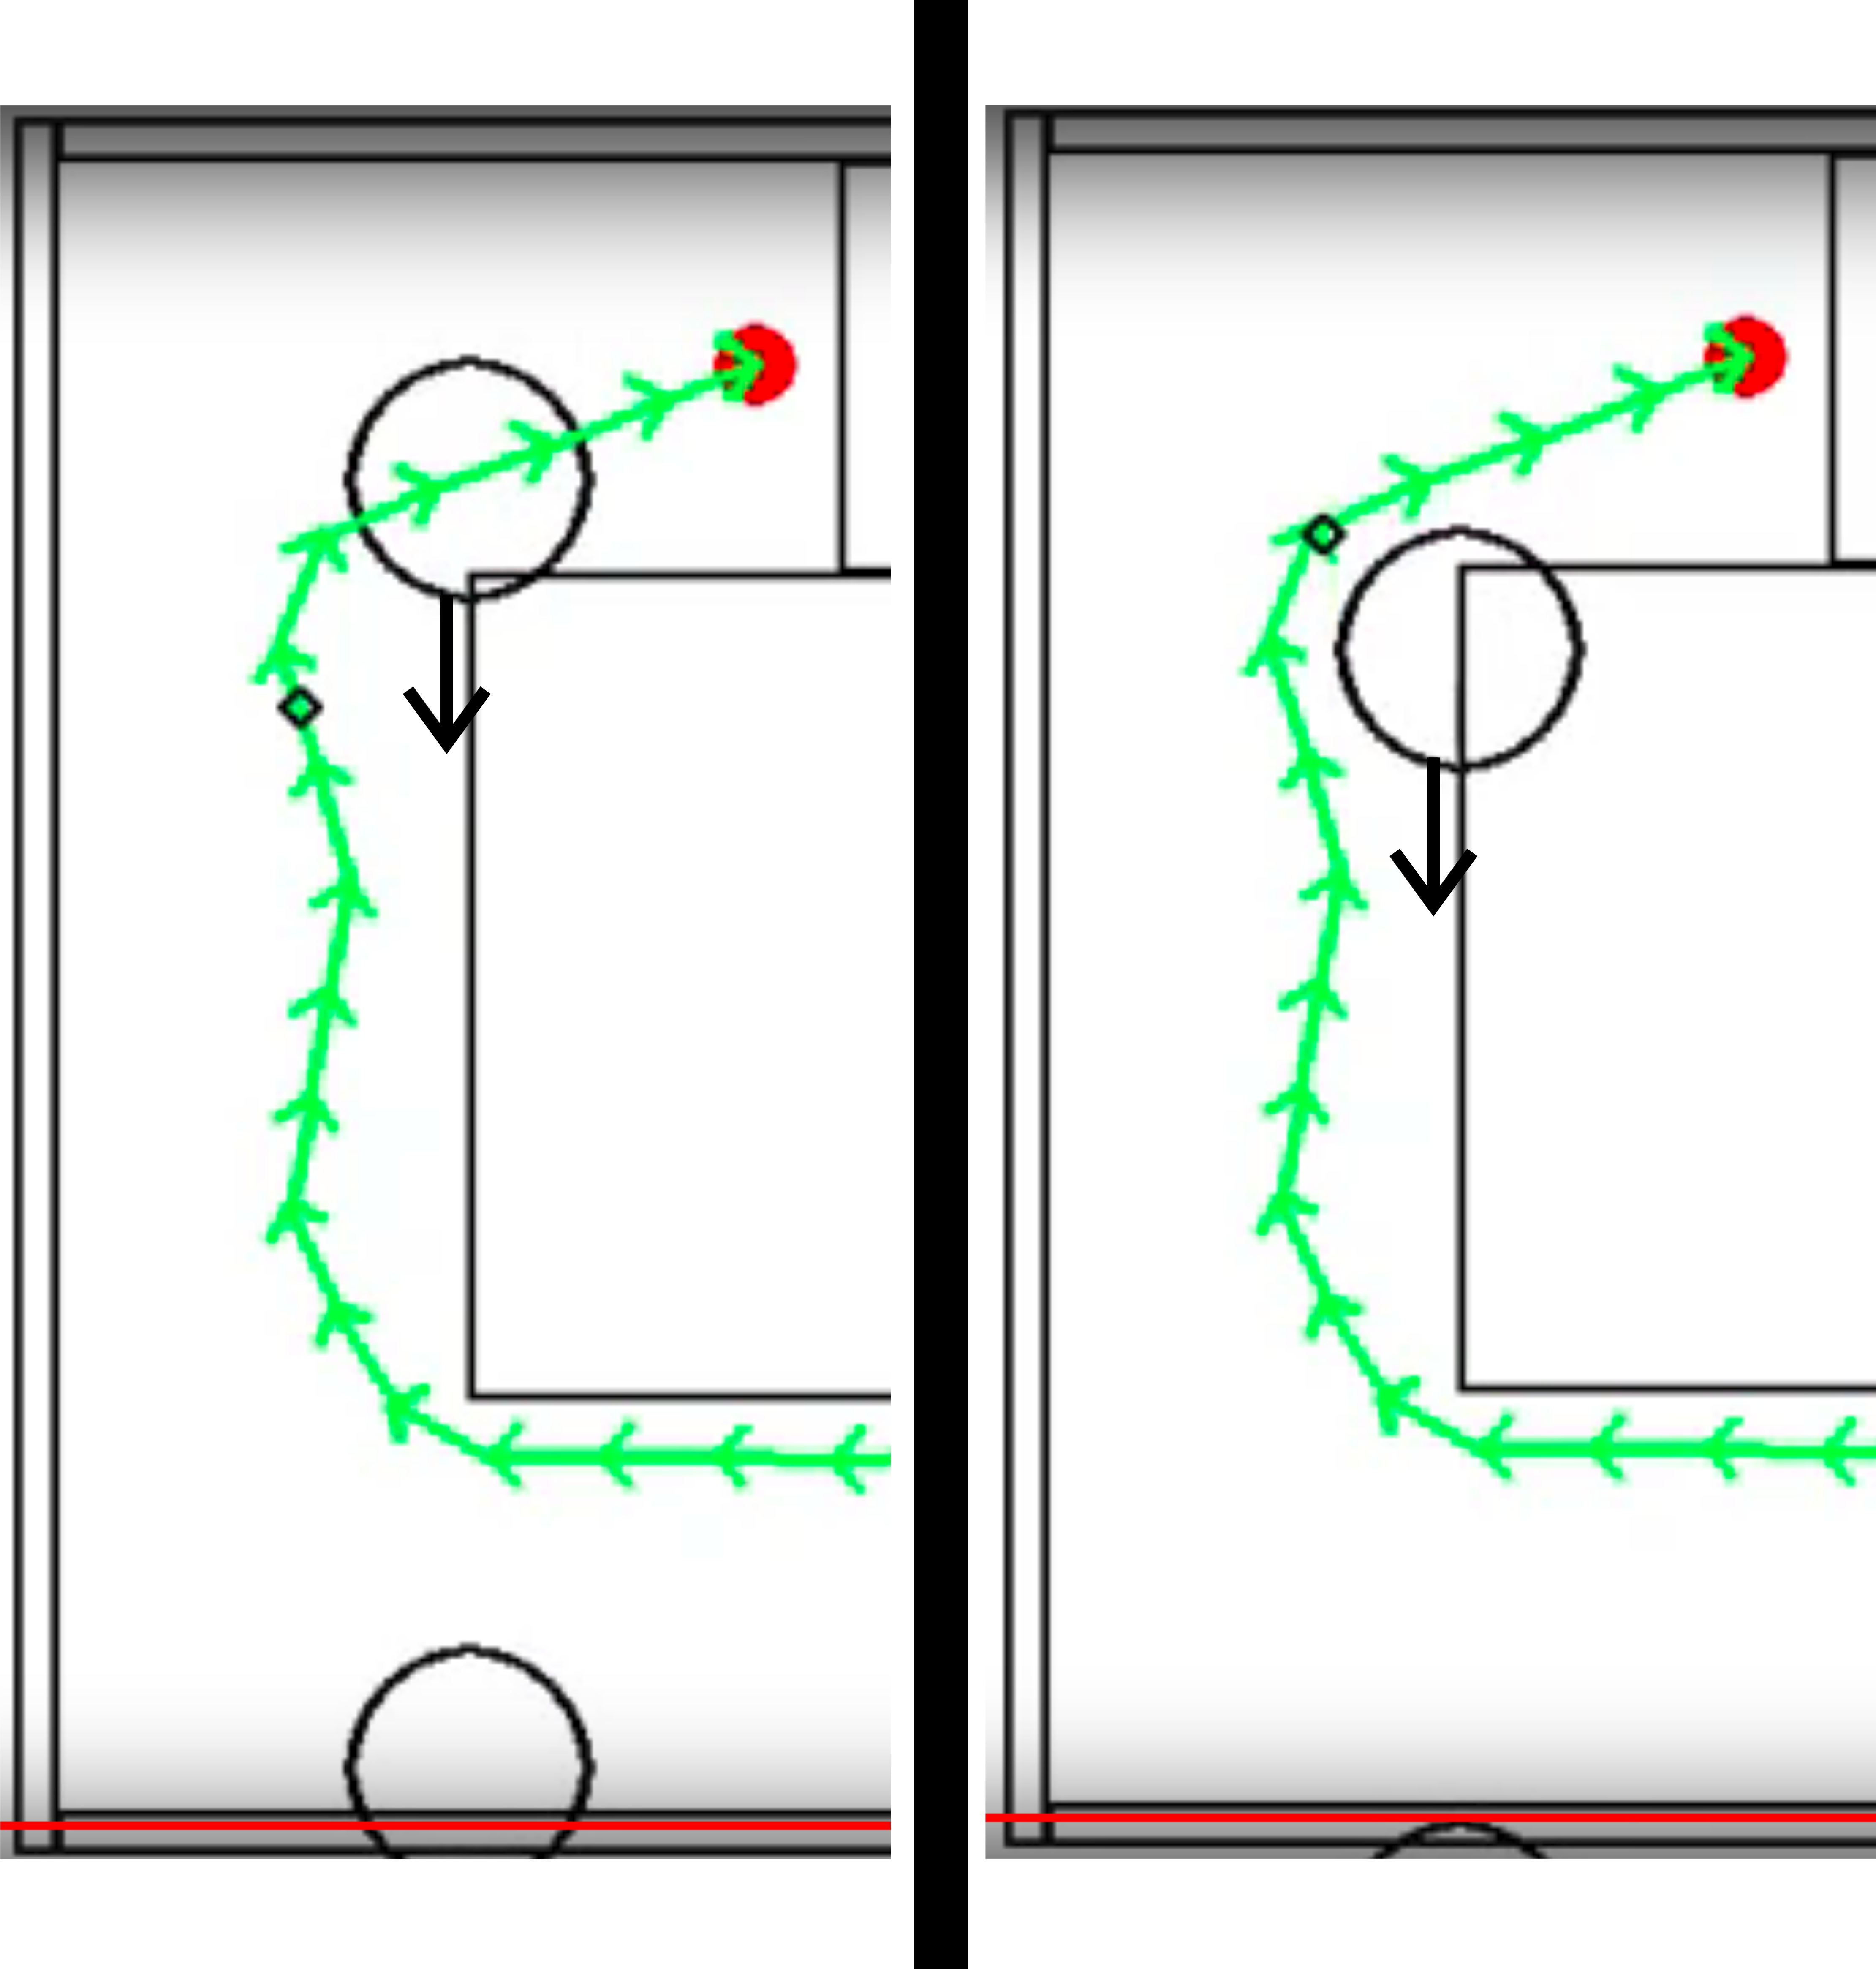
\includegraphics[width=0.5\linewidth]{Figures/07_simulation/moving/dodgeMod2.png}
    \caption{Optimizer adjusts the trajectory and the obstacle is avoided. (time=1m15s)}
    \label{fig:dodM2}
\end{figure}

\par

There is also the need of simulating intruders that do not move with constant speed. For that the trajectory of an aircraft moving in a cluttered map was stored. It was then possible to manually insert an intruder that would follow this trajectory, unknown to the algorithm. The algorithm only knows the position and speed of the intruder with one second of delay, to simulate sensor processing time. Two runs are now shown, in the first one (Figures \ref{nonCoop11}-\ref{nonCoop13}) the intruder is launched later than in the second (Figures \ref{nonCoop21}-\ref{nonCoop23}):




In order to test the limits of the algorithm a 2D simulation was run with an intruder traveling in a zig-zag trajectory towards the aircraft using the produced algorithm. This represents a very challenging situation since the intruder trajectory is constantly changing direction, making it difficult for the algorithm to determine if the aircraft should go above or below the intruder. This simulation was run 10 times and the algorithm failed 4 times (collision happened). One successful simulation is presented in Figures \ref{nonCoop31}-\ref{nonCoop37}.


\begin{figure}[H]
    \centering
    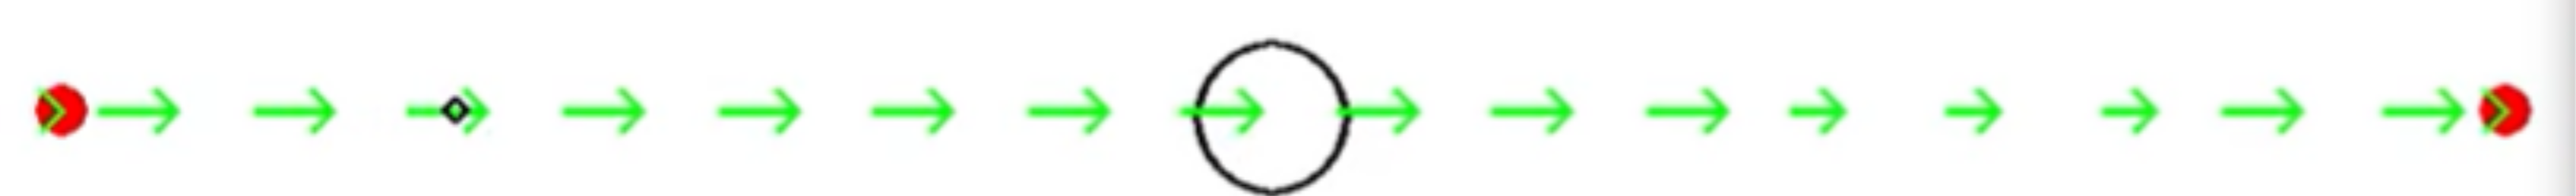
\includegraphics[width=0.7\linewidth]{Figures/07_simulation/nonCoop3/nonCoop31.png}
    \caption{Intruder is detected. As the intruder descends the algorithm doesn't detect a trajectory conflict}
    \label{nonCoop31}
\end{figure}

\begin{figure}[H]
    \centering
    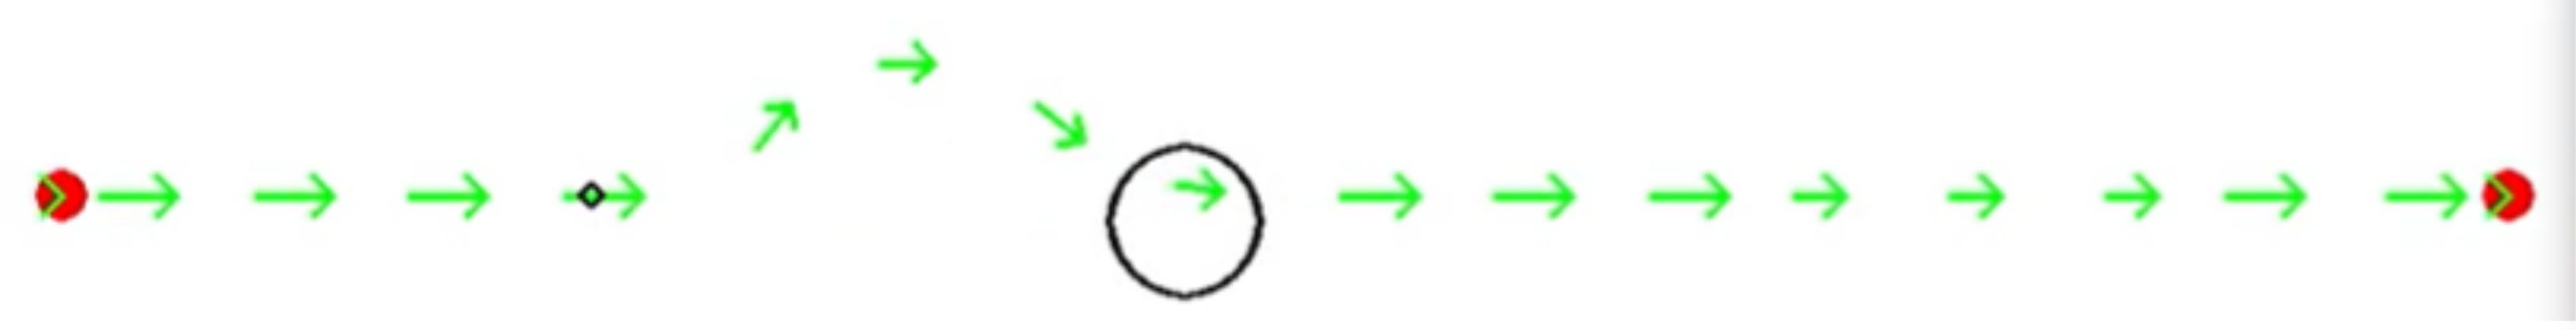
\includegraphics[width=0.7\linewidth]{Figures/07_simulation/nonCoop3/nonCoop32.png}
    \caption{The trajectory is adjusted as the intruder starts to climb}
    \label{nonCoop32}
\end{figure}

\begin{figure}[H]
    \centering
    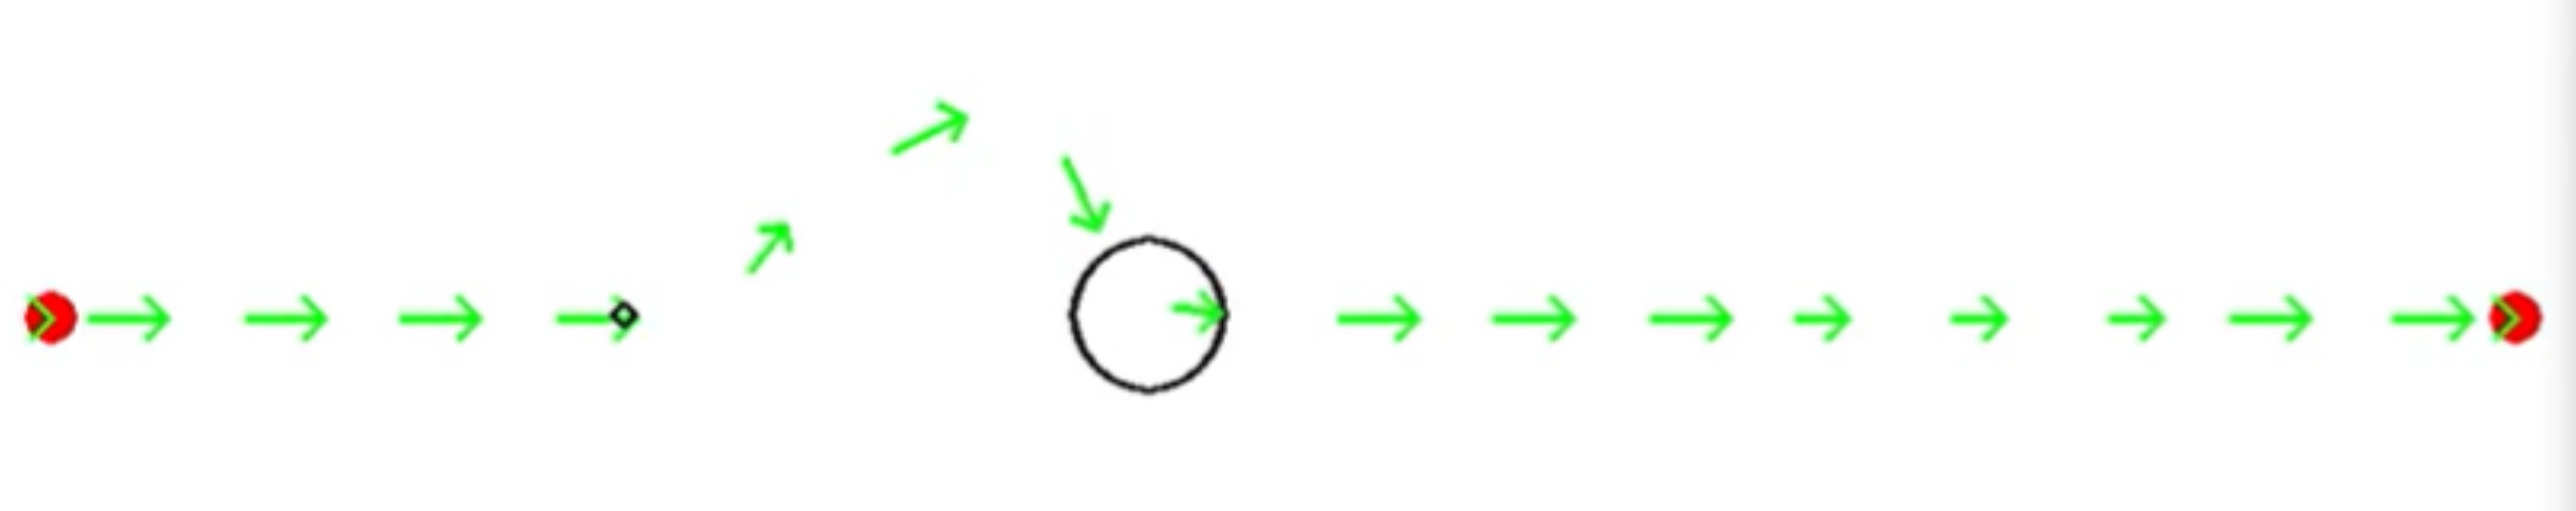
\includegraphics[width=0.7\linewidth]{Figures/07_simulation/nonCoop3/nonCoop33.png}
    \caption{Intruder starts to increase the climb rate. Trajectory is further adjusted.}
    \label{nonCoop33}
\end{figure}

\begin{figure}[H]
    \centering
    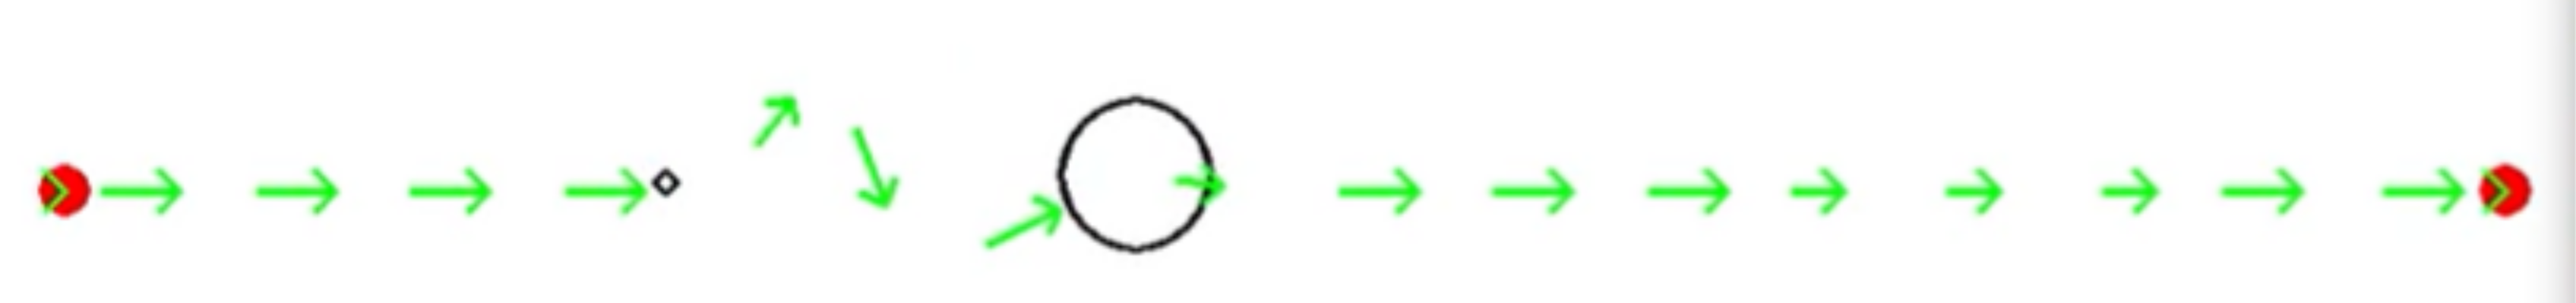
\includegraphics[width=0.7\linewidth]{Figures/07_simulation/nonCoop3/nonCoop34.png}
    \caption{Intruder starts to climb with such a rate that it becomes (apparently) impossible to go above it. Trajectory is adjusted to go under the intruder.}
    \label{nonCoop34}
\end{figure}

\begin{figure}[H]
    \centering
    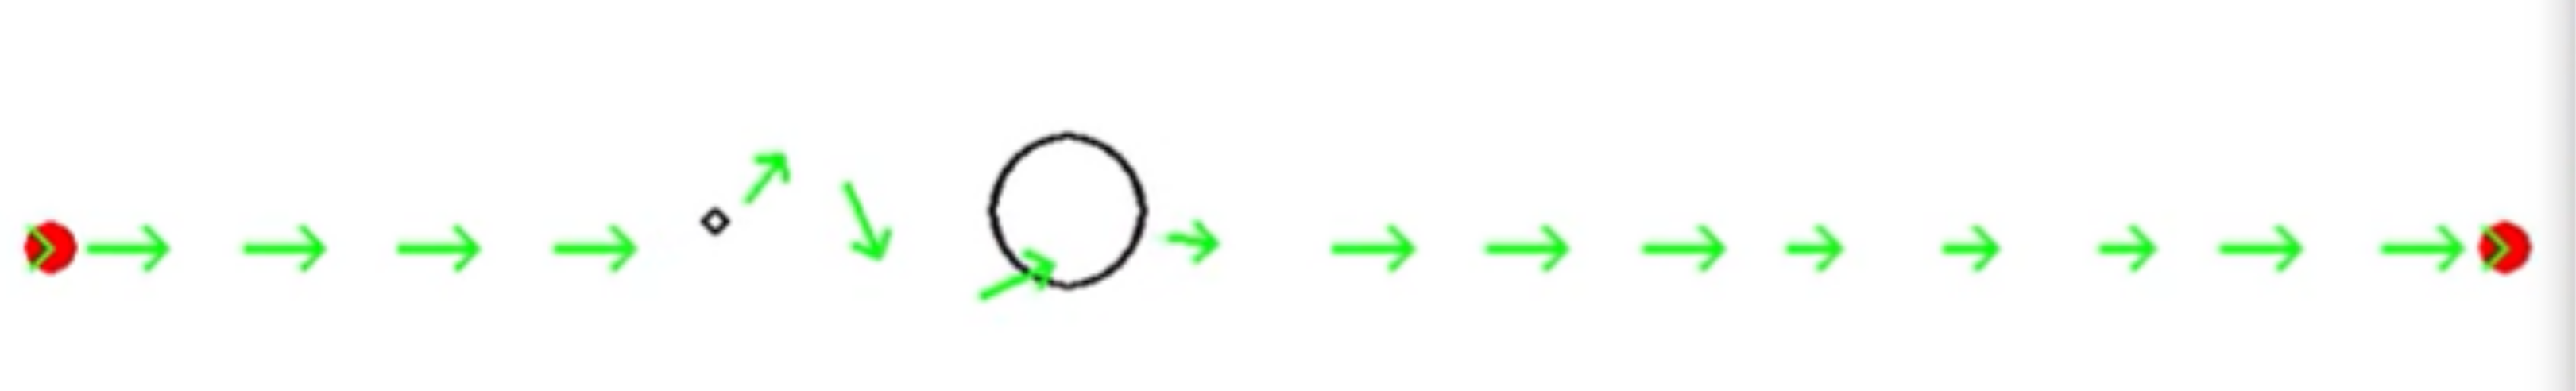
\includegraphics[width=0.7\linewidth]{Figures/07_simulation/nonCoop3/nonCoop35.png}
    \caption{Intruder starts to descend}
    \label{nonCoop35}
\end{figure}

\begin{figure}[H]
    \centering
    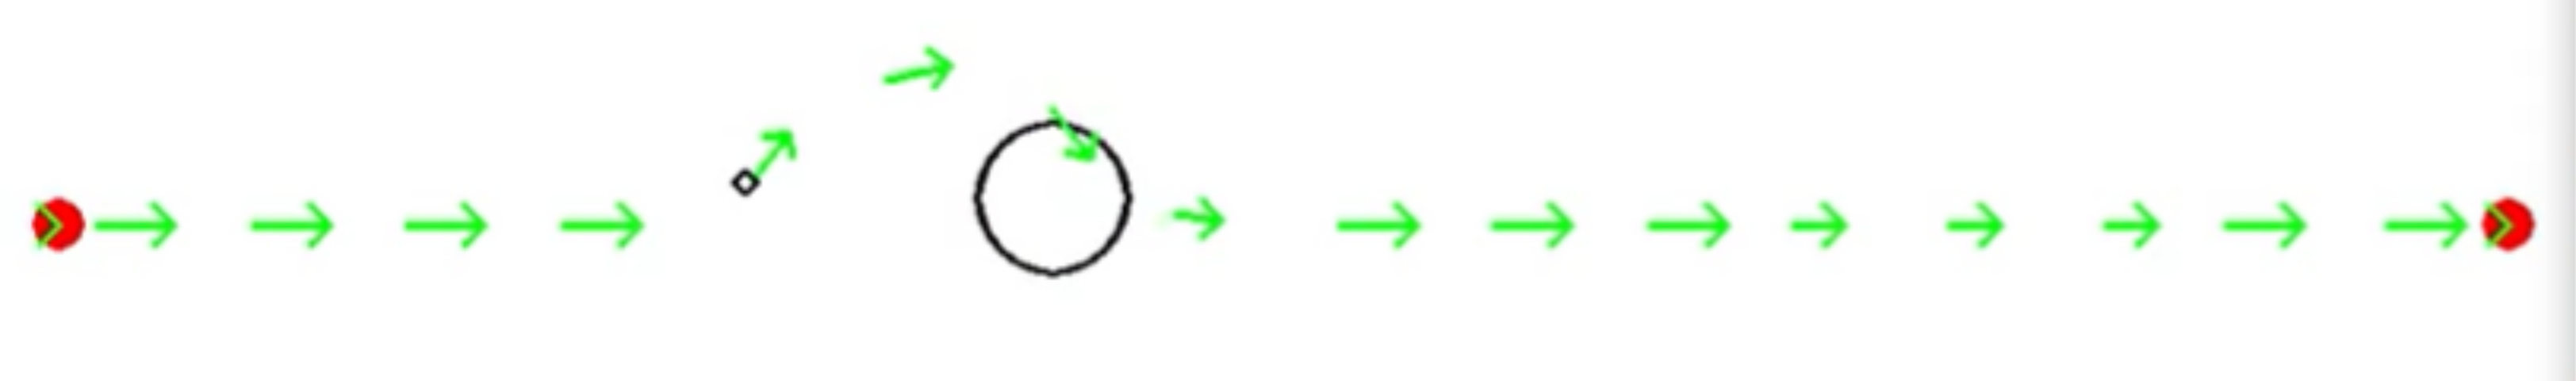
\includegraphics[width=0.7\linewidth]{Figures/07_simulation/nonCoop3/nonCoop36.png}
    \caption{Algorithm (one second later) is informed that intruder is descending and tries to avoid it from above}
    \label{nonCoop36}
\end{figure}

\begin{figure}[H]
    \centering
    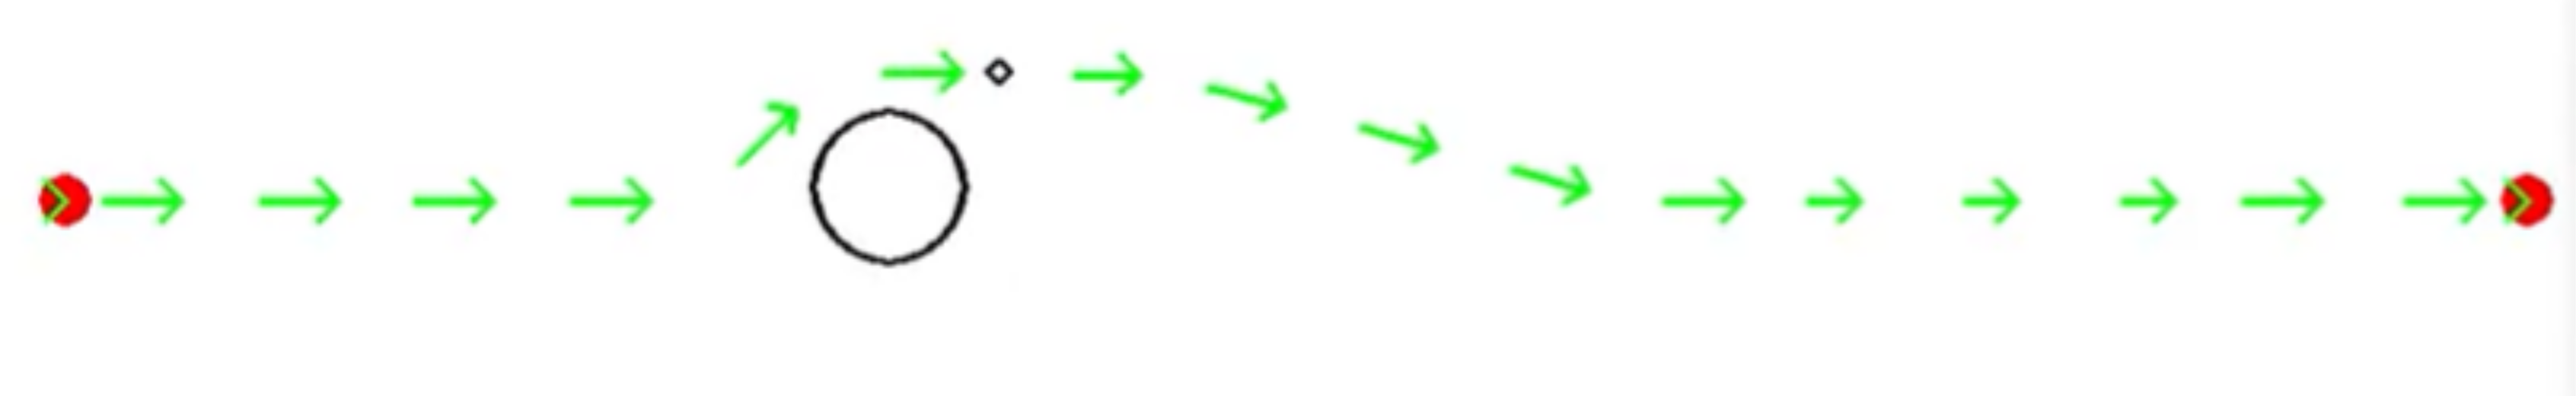
\includegraphics[width=0.7\linewidth]{Figures/07_simulation/nonCoop3/nonCoop37.png}
    \caption{Avoidance is successful}
    \label{nonCoop37}
\end{figure}

\subsection{Simulating an unknown environment}
To simulate an unknown environment the algorithm was used to compute the trajectories in an environment, without knowing the position or number of obstacles in that environment. It was then assumed that the algorithm would acquire information on an obstacle when the aircraft was at a distance to that obstacle smaller than a certain detection range. The evolution of one of these simulations is now shown in Figures \ref{fig:lidar1}-\ref{fig:lidar6}.


To have some statistical data on the performance of the algorithm several simulations were run in random maps, Figures \ref{fig:dodQ} show one of these random maps.

\begin{figure}[H]
    \centering
    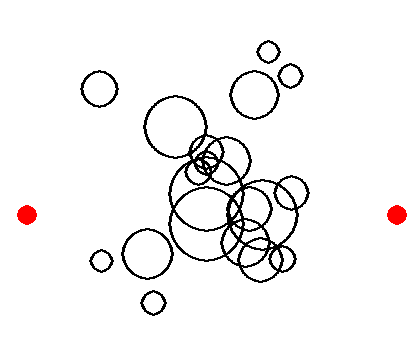
\includegraphics[width=0.6\linewidth]{Figures/07_simulation/lidar/lidarRandQ.png}
    \caption{Random unknown map.}
    \label{fig:dodQ}
\end{figure}


Each map has 20 randomly generated circles, with a radius between 10 and 40 (display units). The distance from start to goal was 370 display units. Table \ref{tab:randomResults} shows the time taken to reach the goal and the number of times the trajectory was fully or partially regrown. The algorithm wasn't able to compute a trajectory once, in that case the aircraft stopped at a distance smaller than the safe distance, relatively to an obstacle. For that reason the RRT algorithm could not output any safe trajectory.


\begin{table}[]
    \centering
    \begin{tabular}{c|cc}
        attempt & number of regrows & time \\ \hline
        1 & 0 &  34 (s) \\
        2 & 0 &  32 (s) \\
        3 & 0 &  36 (s) \\
        4 & 2 &  62 (s) \\
        5 & 1 &  46 (s) \\
        6 & 0 &  32 (s) \\
        7 & 3 &  -  \\
        8 & 0 &  39 (s) \\
        9 & 0 &  47 (s) \\
        10& 1 &  49 (s) \\ \hline
        
        
    \end{tabular}
    \caption{Results of the runs in random maps.}
    \label{tab:randomResults}
\end{table}{}

\subsection{Multi-Aircraft}
In a realistic scenario several aircrafts share the same air-space. In a future where urban transportation is also accomplished using aircrafts the algorithms must prove to enable safe circulation. Once this work aims for a decentralized approach it is expected that algorithms running independently in several aircrafts are able to provide collision free paths, without a centralized entity taking a decision. The aircraft, in this simulation, share their flight plan.
\par
The experiment was conducted 10 times in a scenario where two aircrafts must coordinate the passage through a narrow gap. In all of the trials there were no collisions. The results are shown on Fig. \ref{fig:twoAir0} - \ref{fig:twoAir2}.

The experiment was repeated when one of the aircraft ignores the presence of the other. This resembles a scenario where one of the aircraft has priority over the other and, therefor, flies unconcerned. This experiment was also successful in the 10 trials.

\subsection{Physics simulation}
The previous algorithms were developed taking as assumptions that the UAV could be described as a body subjected to forces as inputs. The resulting trajectories are a sequence of constant acceleration segments. Such a formulation of the problem leads to the existence of discontinuities in the acceleration. A physical multi-rotor can not, however, provide discontinuities in the acceleration, even if it is considered that the rotor velocities can change instantaneously. For this reason many works use polynomials with higher degrees, in order to provide continuity of the acceleration and jerk (3rd derivative of the position).   This is associated to the fact that the multi-rotor can only produce thrust in the axis perpendicular to the rotors’ plane, meaning that discontinuities in the acceleration and jerk would correspond to discontinuities in the multi-rotor attitude and angular rate respectively.  In \cite{ETH} and \cite{agressive} the authors use 11th and 9th order polynomials for computing the trajectories, respectively. In \cite{ref:quad} the authors use a spline that assures continuity up to the 4th derivative of the position for smoothing the trajectory.
\par
It is clear that there is a need to verify the capability of a multi-rotor with realistic dynamics to follow the computed trajectories, once the simplified model used to validate the real-time capability of the algorithms doesn't rigorously approximate a real UAV.
\par
For simulating it will be used the Robotics Operative System (ROS) \cite{ref:ROS} and the physics engine Gazebo \cite{ref:Gazebo}. A plugin for Gazebo, RotorS, was developed in the Autonomous Systems Lab of ETH Zurich university \cite{Furrer2016}. This plugin includes multi-rotor models and example controllers, that are used in the current work. This open source simulator also has the advantage of enabling the simulation of a variety of sensors and allow a posterior straight forward  implementation in real multi-rotors.
\par
The controller for the simulated aircraft was adapted from the one described in the work by Lee et al. \cite{Lee}. Changes were made to allow the controller to predict the references while the trajectory planner does not update them.
\par
It was chosen a simple map for validation of the algorithm. The map consisted of a gazebo model of a fast-food chain restaurant. Fig. \ref{mapPrespectiveSim} represents the simulation scenario. The algorithm computes a trajectory from one of the sides of the building to the other.

\begin{figure}[!ht]
    \centering
    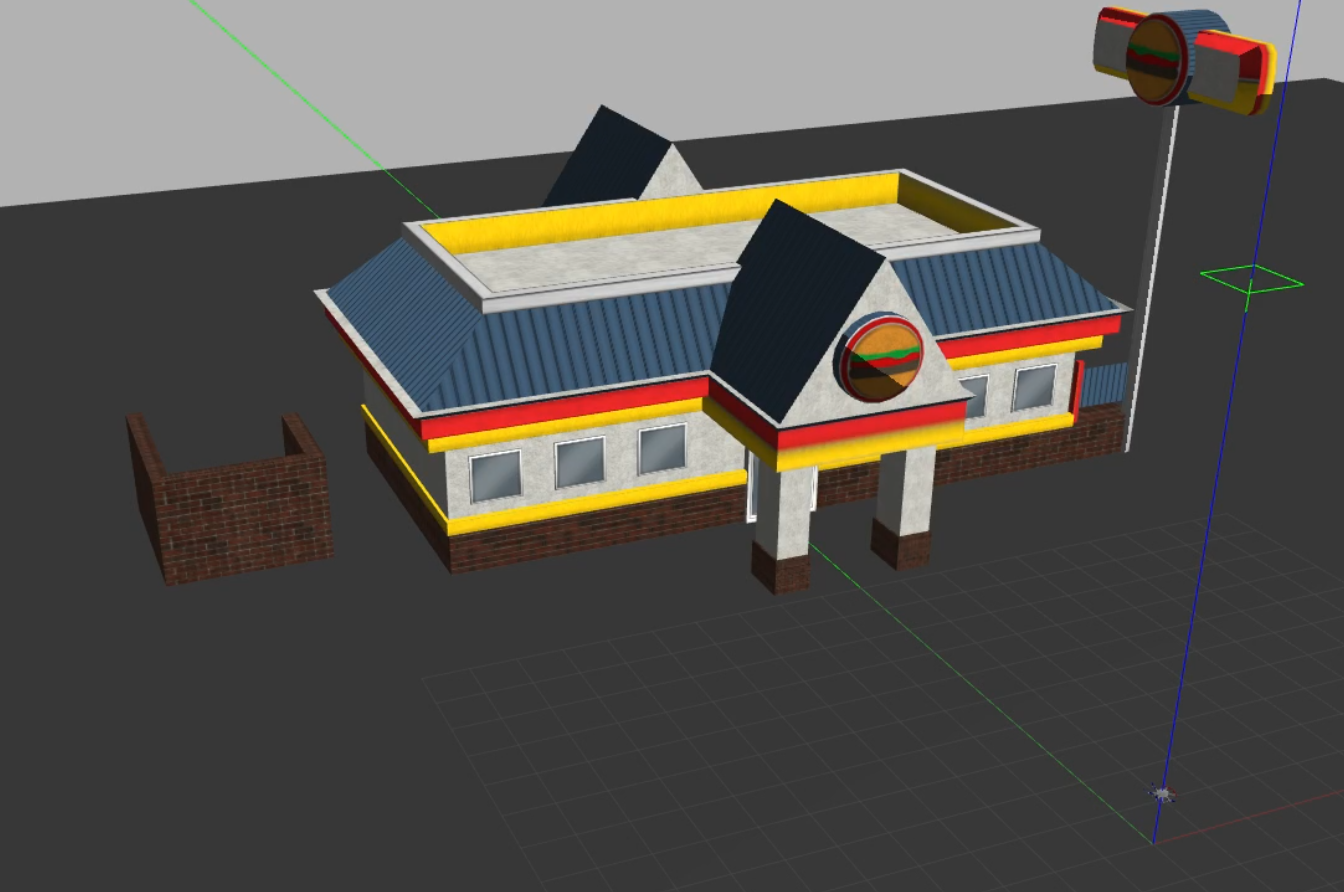
\includegraphics[width=0.9\linewidth]{Figures/07_simulation/Sim/mapGazebo.png}
    \caption{Map visualization on the Gazebo simulator environment}
    \label{mapPrespectiveSim}
\end{figure}

Four runs were performed. The results of four runs are now presented. The runs differ in maximum acceleration allowed and the side of the building taken to arrive to the goal position. In all the runs the minimum distance allowed between the UAV and an obstacle was set to 3 meters and the maximum speed allowed for the UAV to travel was 15 $m$/$s$ ( 54 km/h). For run 1 and 2 the maximum allowed acceleration was 6$m$/$s^2$ and for run 3 and 4 10$m$/$s^2$.

The trajectory taken by the vehicle in one of the runs (run 3) is presented in Fig. \ref{trajRun3}.

\begin{figure}[ht!]
    \centering
    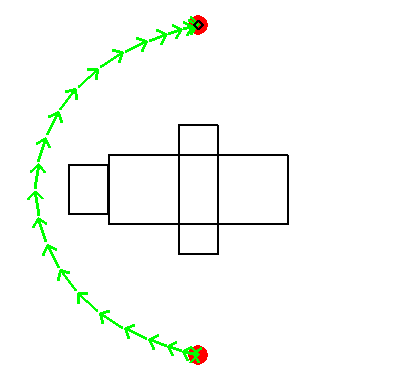
\includegraphics[width=0.6\linewidth]{Figures/07_simulation/Sim/trajL10.png}
    \caption{Trajectory taken in run 3 (Max. acceleration = 10$m$/$s^2$).}
    \label{trajRun3}
\end{figure}

The norm of the difference between the aircraft position and the reference position provided by the algorithm was stored over time for every time an update was received on the aircraft position. The evolution of the position error along the time is now presented for run 3 in Fig. \ref{alongRun3}.

\begin{figure}[H]
    \centering
    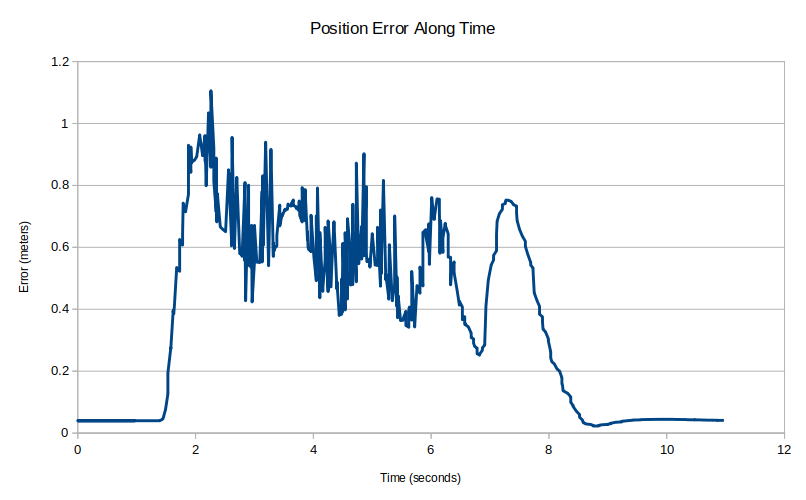
\includegraphics[width=0.9\linewidth]{Figures/07_simulation/Sim/L10along.png}
    \caption{Position error along the simulation time in run 3 (Max. acceleration = 10$m$/$s^2$).}
    \label{alongRun3}
\end{figure}

It is possible to observe in Fig. \ref{alongRun3} that the position error is low and stabilized while the UAV is hovering, before and after executing the trajectory. The error doesn't tend to zero because the controller expression doesn't contain an integral term. During the trajectory execution the position error rises but it is never greater than one meter except for brief moments in run 3. As expected measured error was greater when the maximum acceleration allowed is greater (for runs 3 and 4).

\begin{figure*}[!htb]
    \centering
    \begin{minipage}[b]{.3\linewidth}
        \centering
        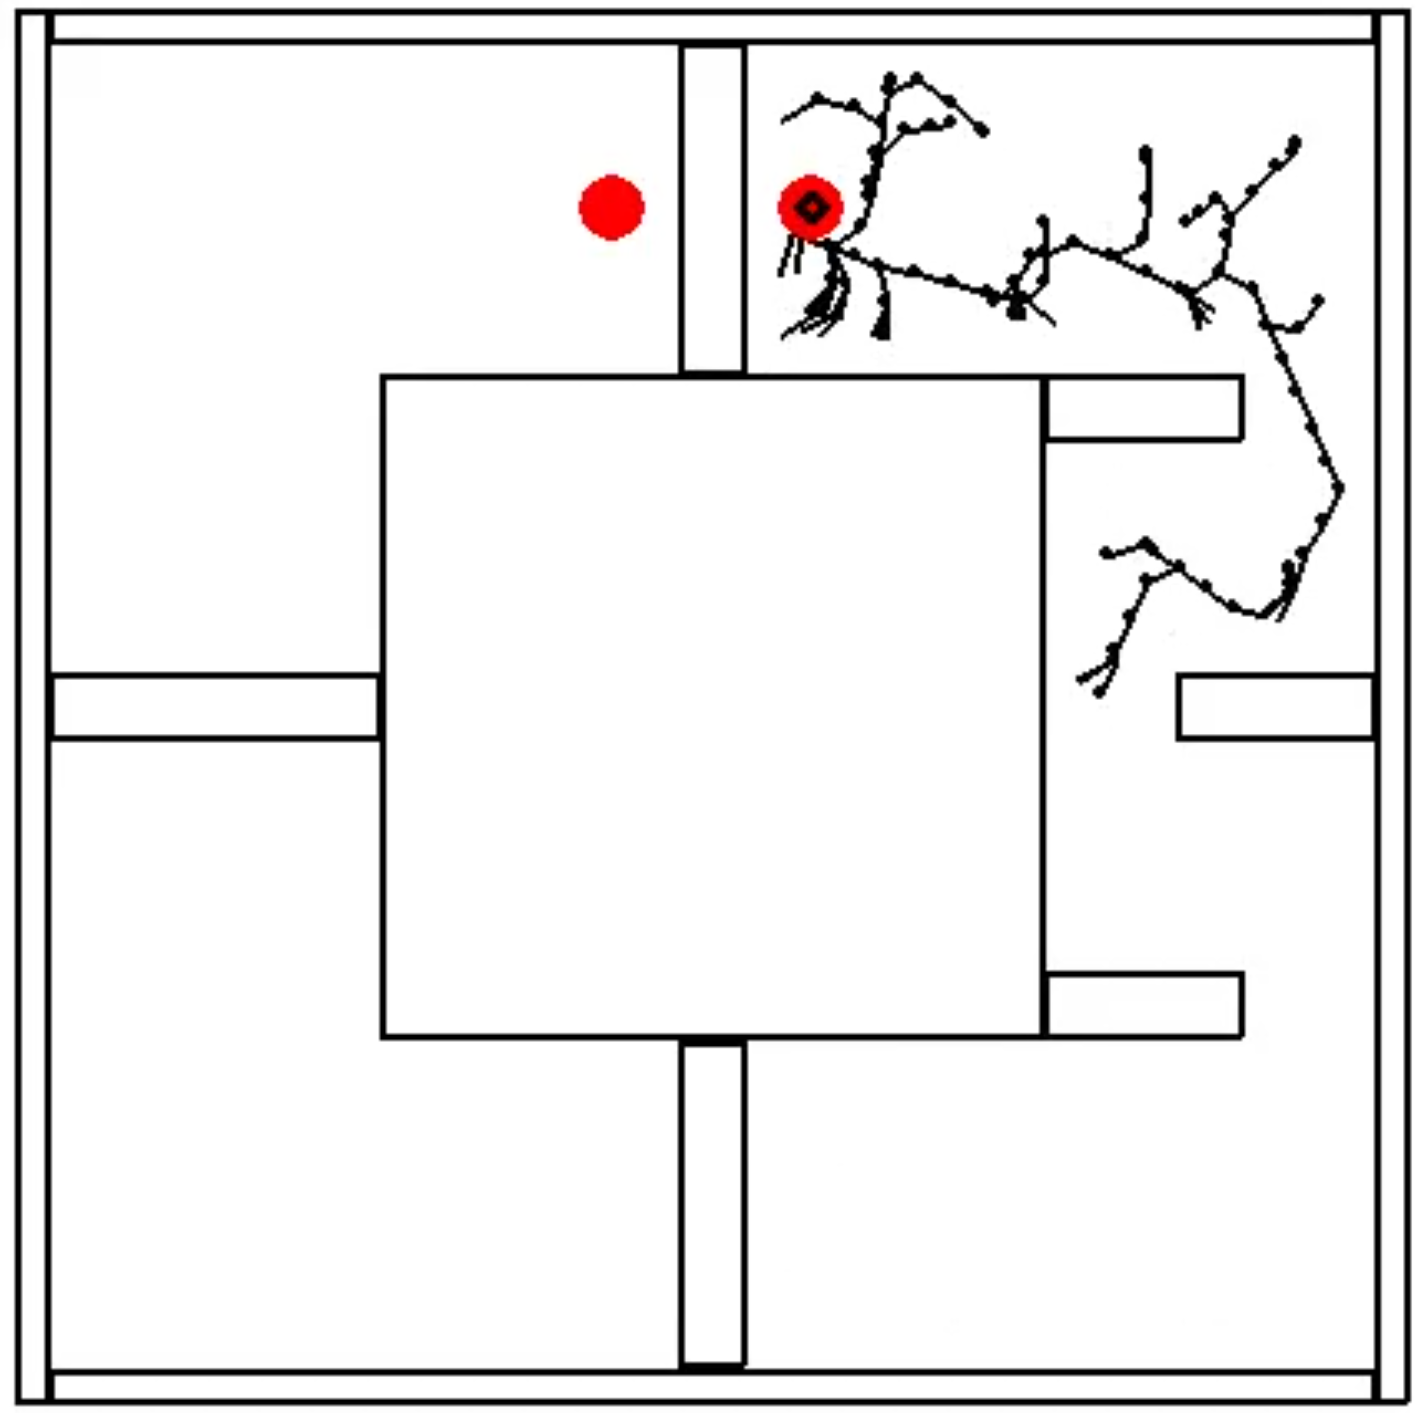
\includegraphics[width=0.8\linewidth]{Figures/07_simulation/basic/00basic.png}
    \end{minipage}%
    \hfill%
    \begin{minipage}[b]{.3\linewidth}
        \centering
        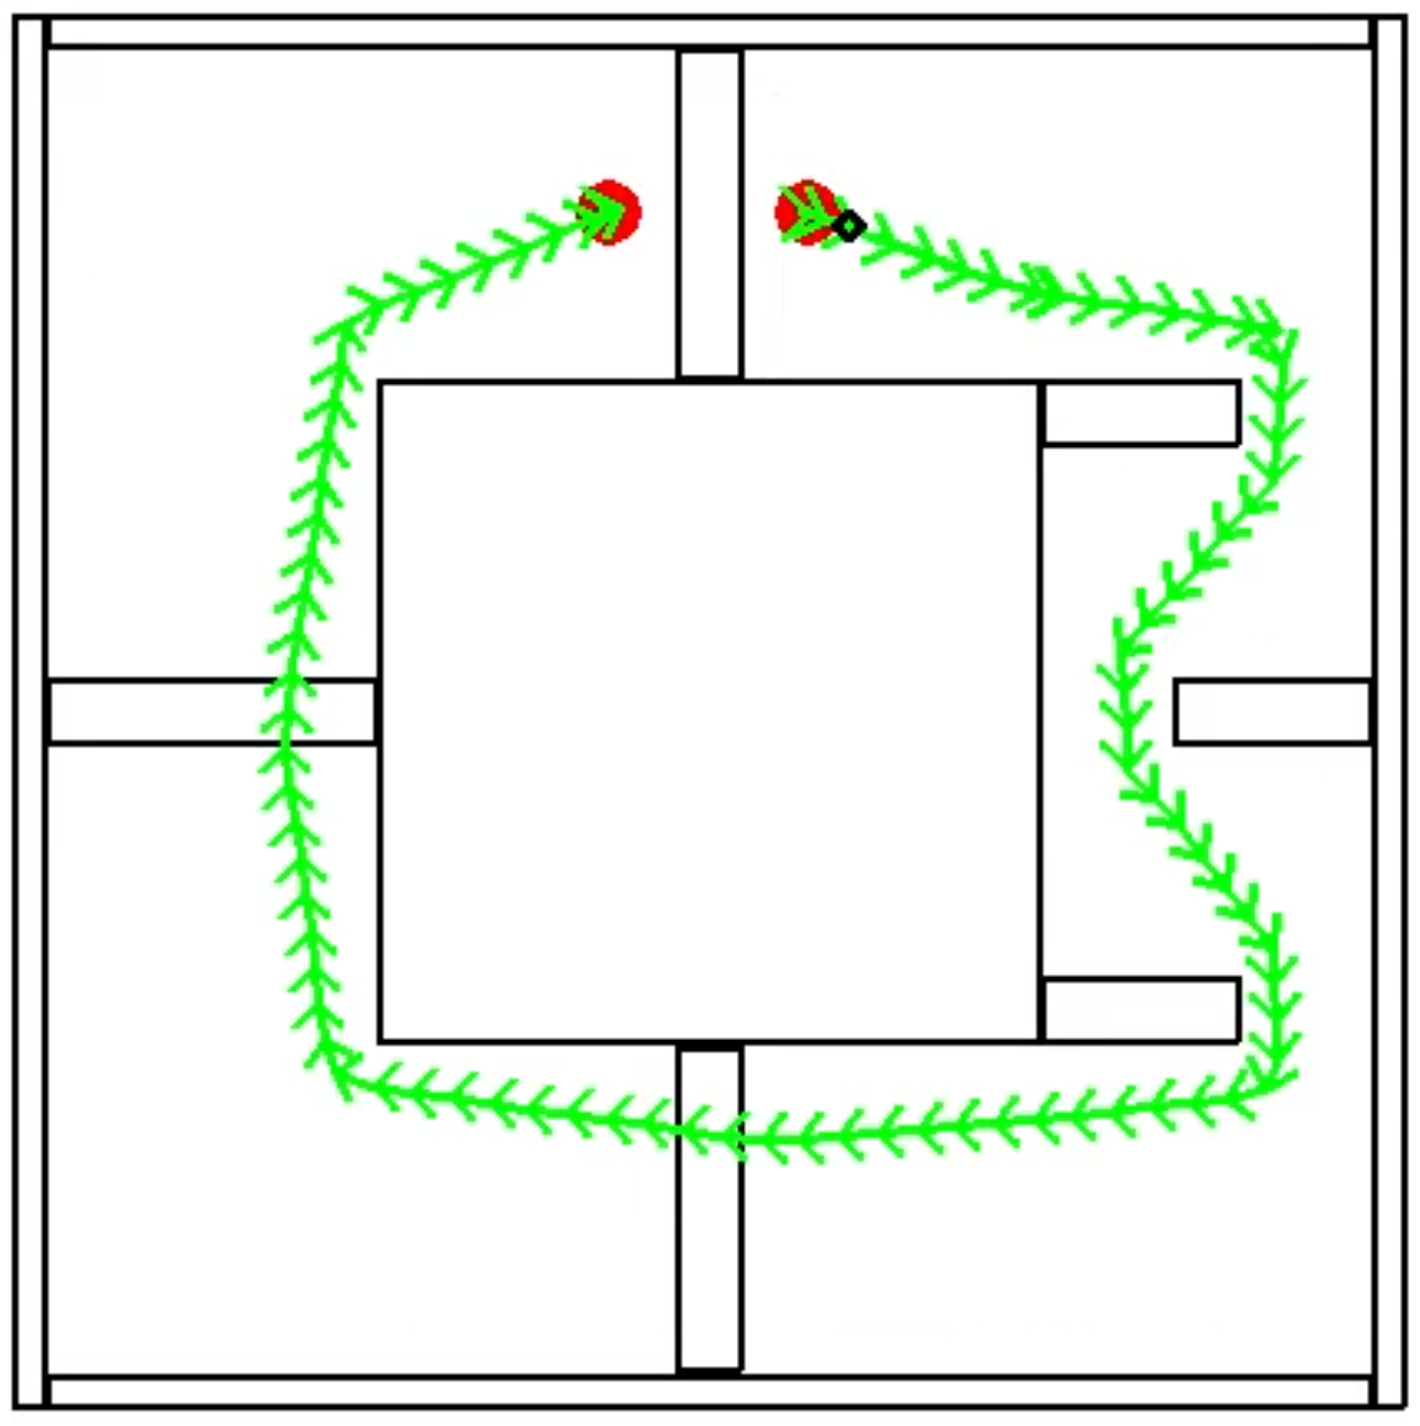
\includegraphics[width=0.8\linewidth]{Figures/07_simulation/basic/01basic.png}
    \end{minipage}%
    \hfill%
    \begin{minipage}[b]{.3\linewidth}
        \centering
        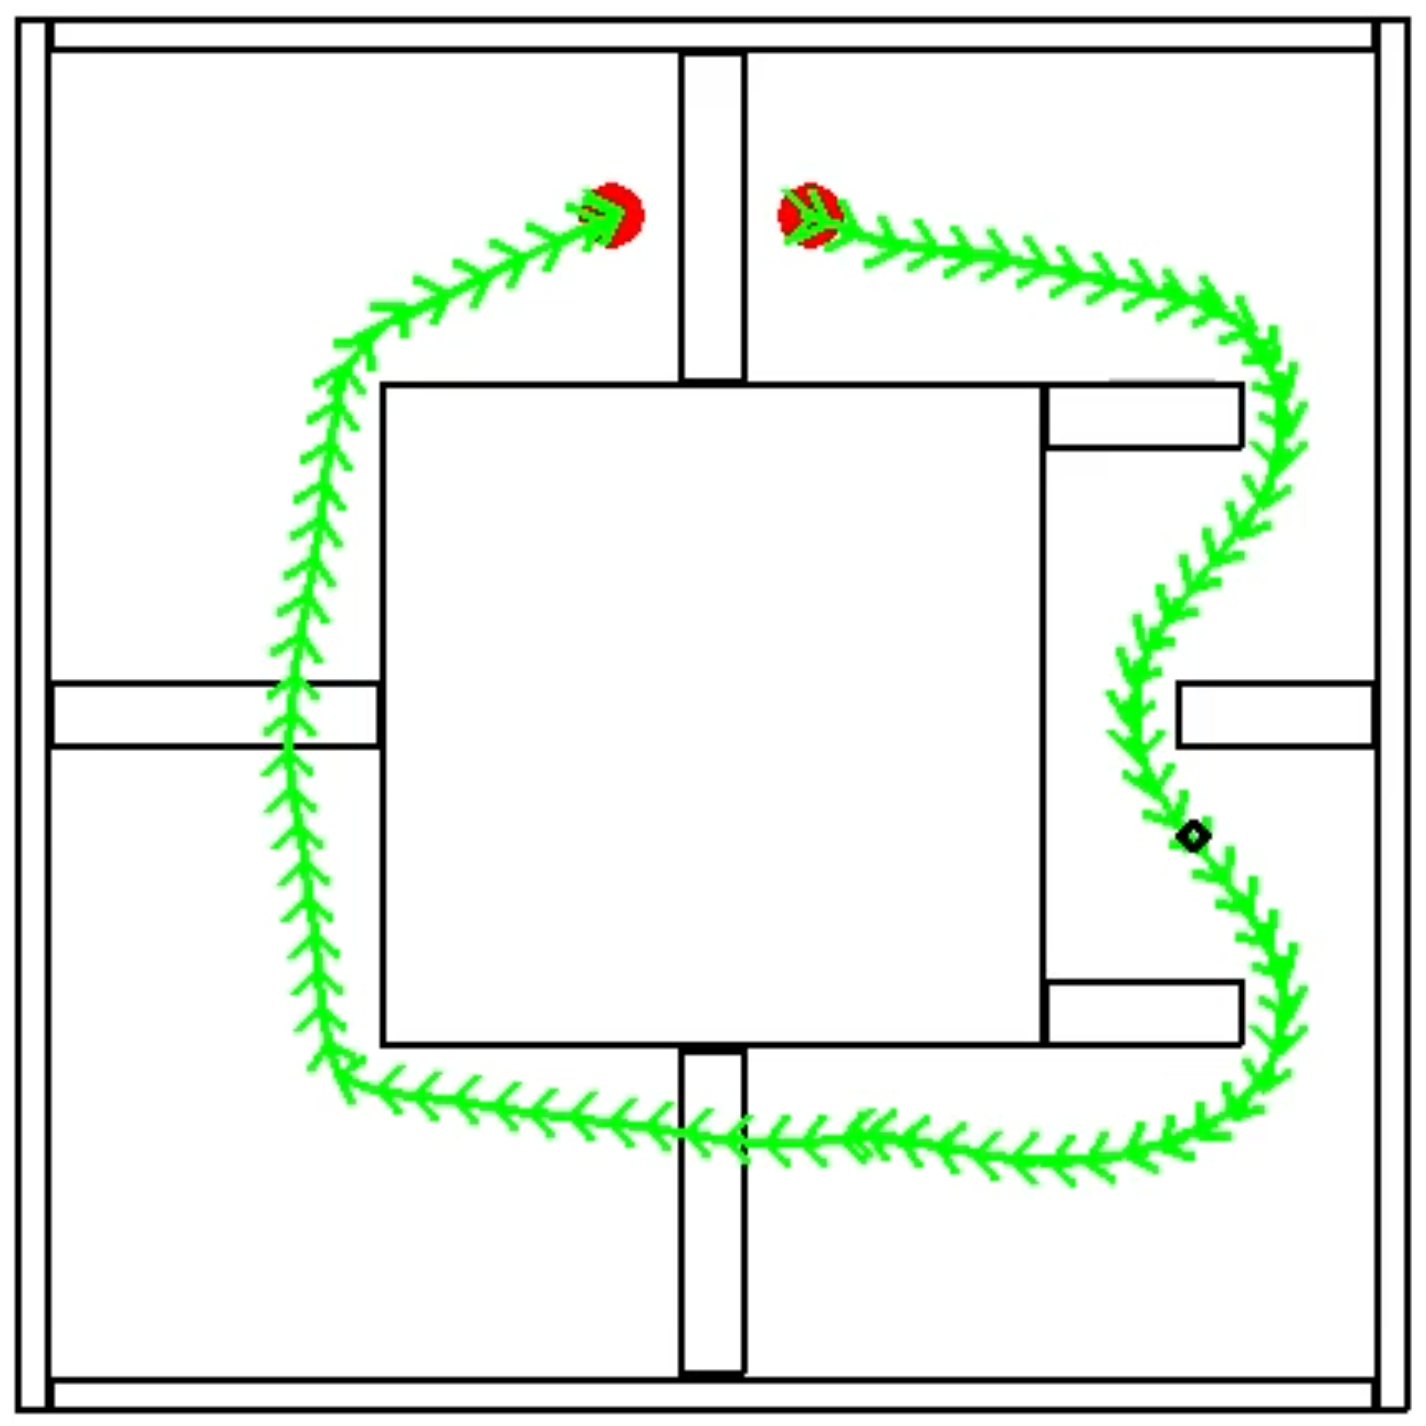
\includegraphics[width=0.8\linewidth]{Figures/07_simulation/basic/03basic.png}
    \end{minipage}\\[-7pt]
    \begin{minipage}[t]{.3\linewidth}
    \caption{RRT is grown (t=0s)}
    \label{fig:basic00}
    \end{minipage}%
    \hfill%
    \begin{minipage}[t]{.3\linewidth}
    \caption{Initial trajectory is computed (t=3s)}
    \label{fig:basic01}
    \end{minipage}%
    \hfill%
    \begin{minipage}[t]{.3\linewidth}
    \caption{The algorithm optimizes part of the trajectory ahead of the aircraft.}
    \label{fig:basic03}
    \end{minipage}%
\end{figure*}

\begin{figure*}[!htb]
    \centering
    \begin{minipage}[b]{.3\linewidth}
        \centering
        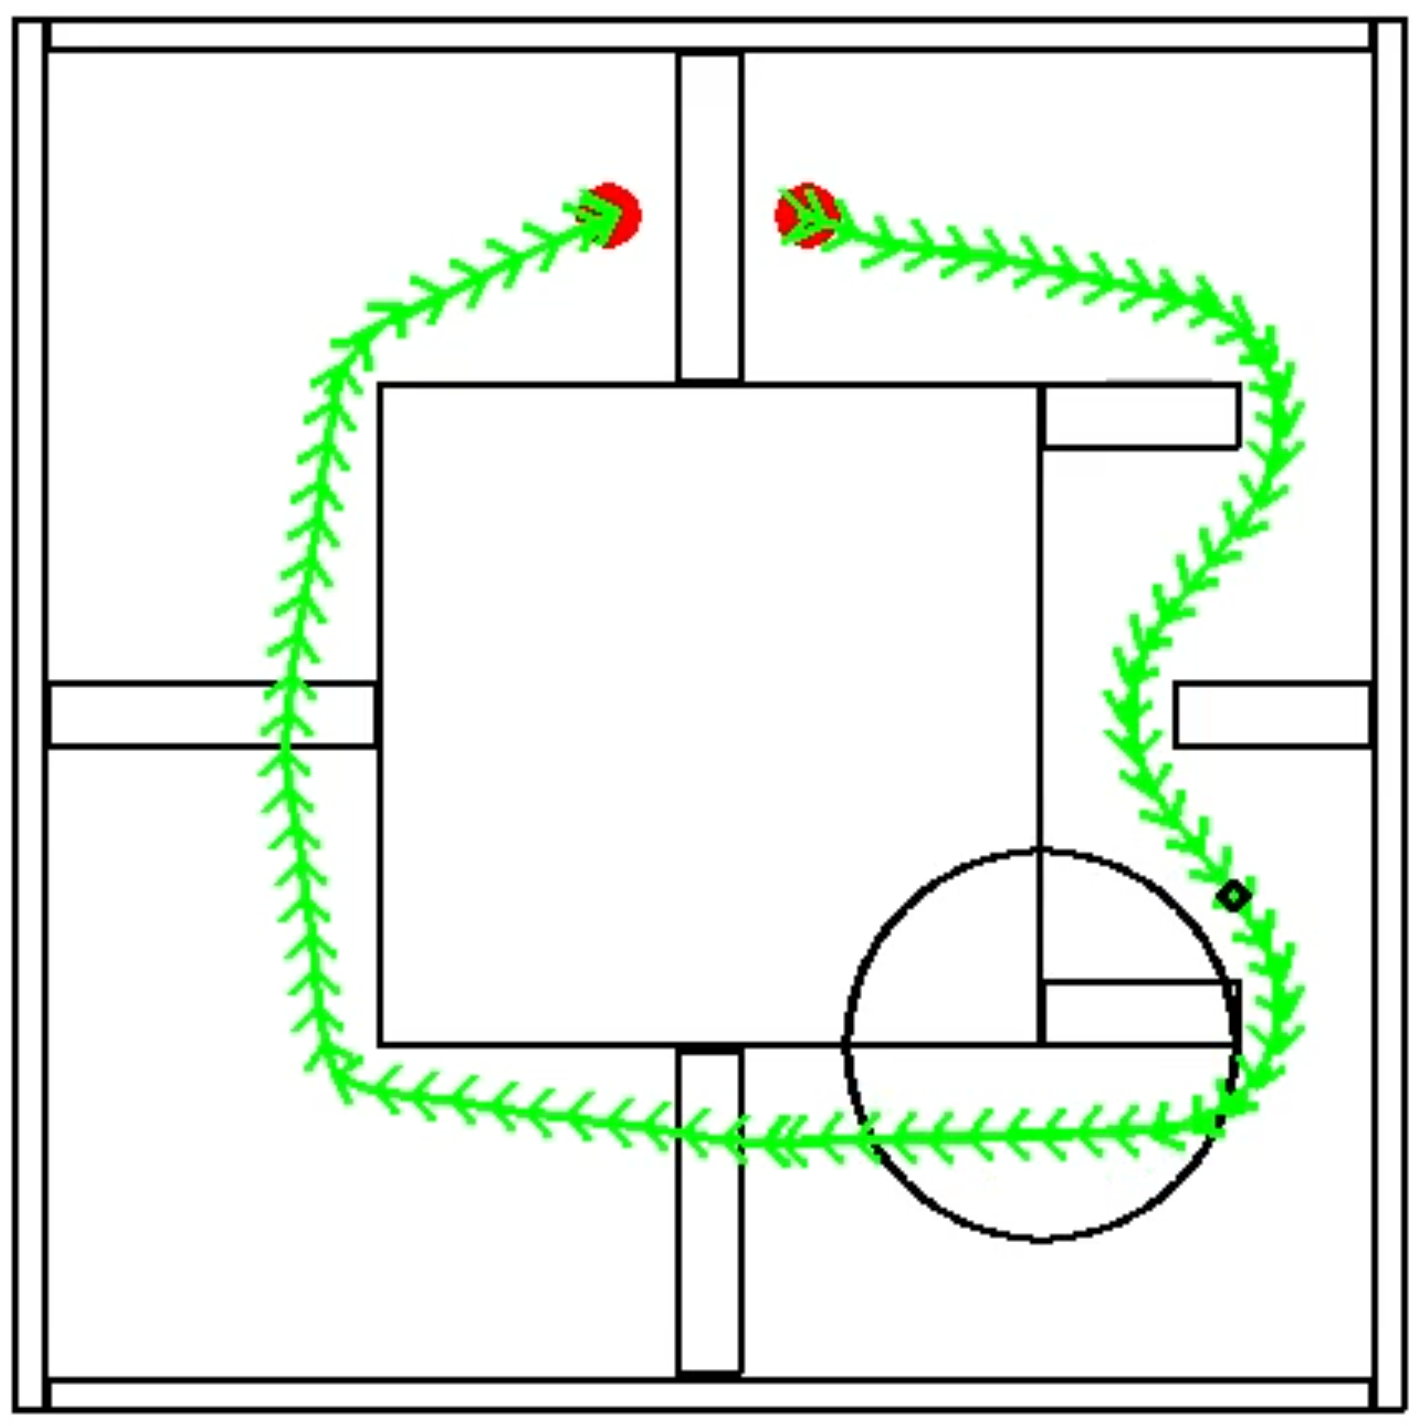
\includegraphics[width=0.8\linewidth]{Figures/07_simulation/basic/04basic.png}
    \end{minipage}%
    \hfill%
    \begin{minipage}[b]{.3\linewidth}
        \centering
        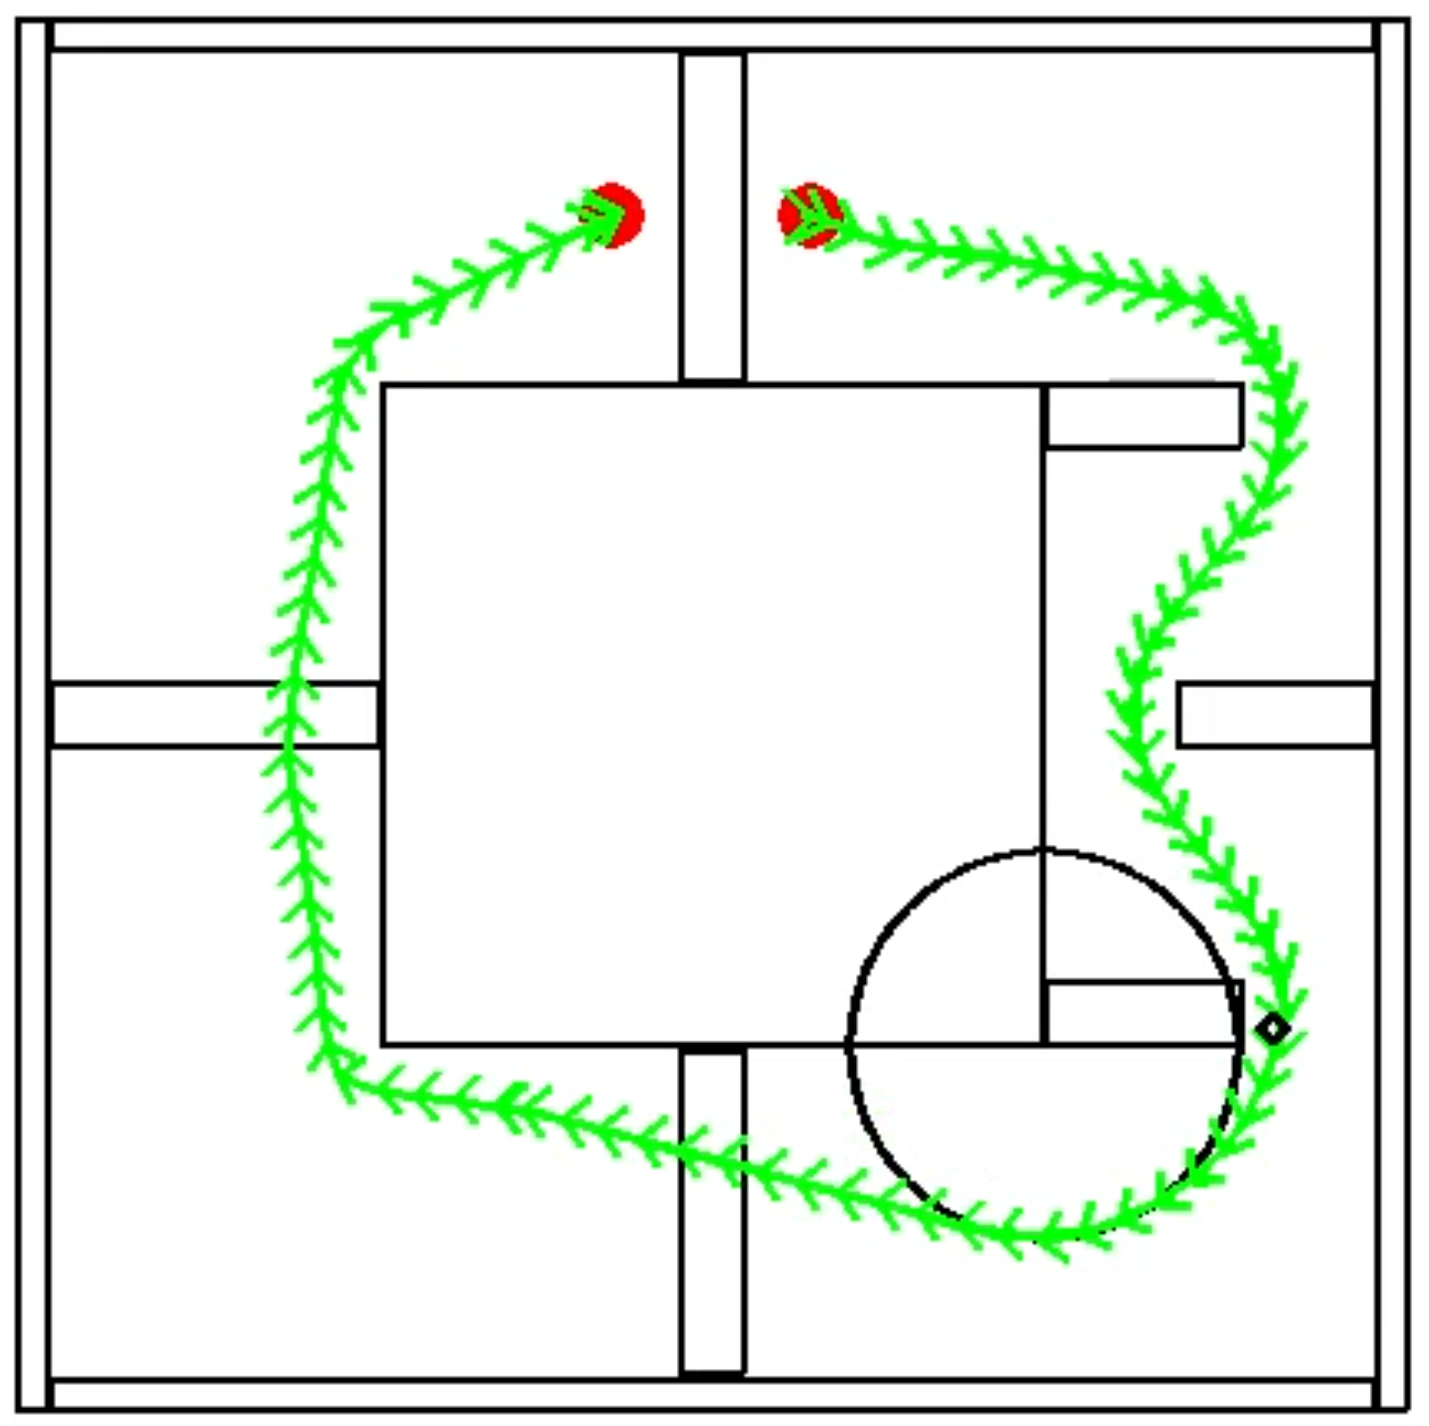
\includegraphics[width=0.8\linewidth]{Figures/07_simulation/basic/05basic.png}
    \end{minipage}%
    \hfill%
    \begin{minipage}[b]{.3\linewidth}
        \centering
        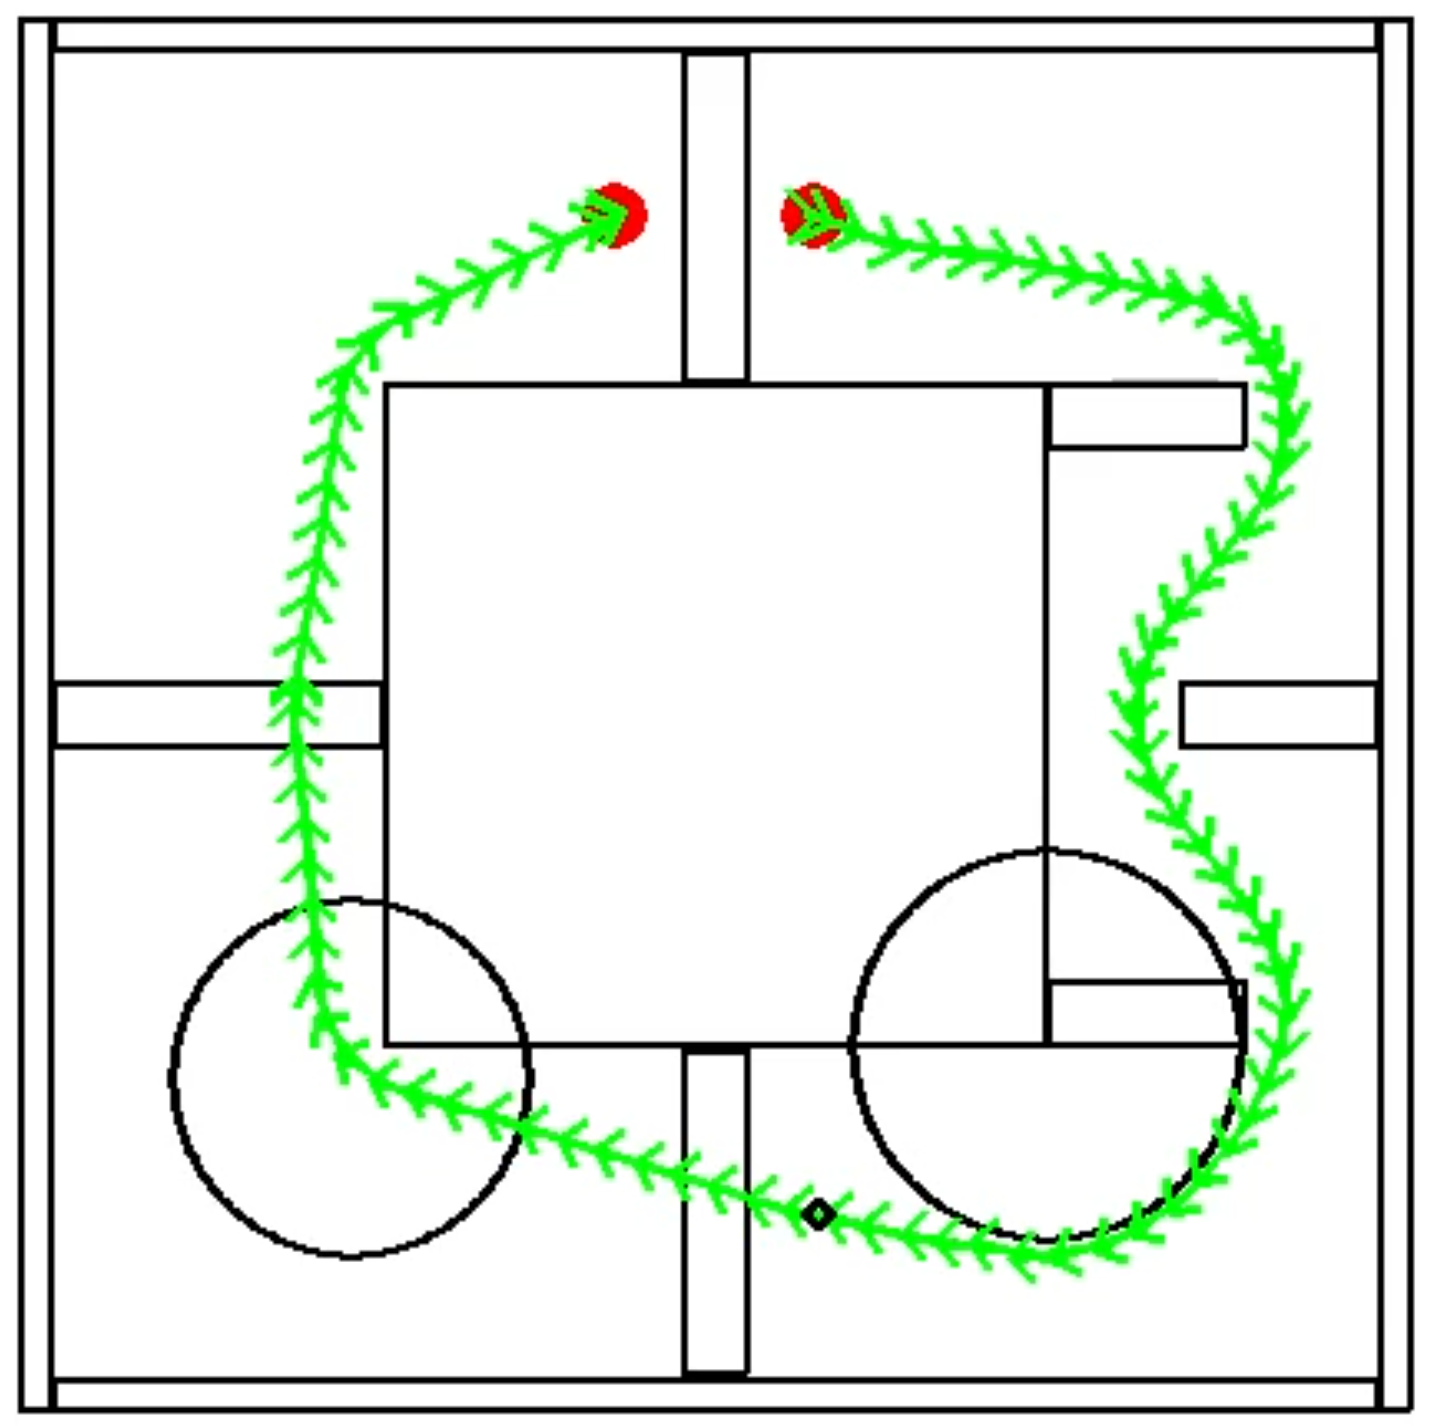
\includegraphics[width=0.8\linewidth]{Figures/07_simulation/basic/07basic.png}
    \end{minipage}\\[-7pt]
    \begin{minipage}[t]{.3\linewidth}
        \caption{Obstacle is detected (t=25s) }
        \label{fig:basic04}
    \end{minipage}%
    \hfill%
    \begin{minipage}[t]{.3\linewidth}
        \caption{Trajectory optimizer adjusts the trajectory avoiding the obstacle (t=27s)}
        \label{fig:basic05}
    \end{minipage}%
    \hfill%
    \begin{minipage}[t]{.3\linewidth}
        \caption{Obstacle is detected  (t=41s)}
        \label{fig:basic07}
    \end{minipage}%
\end{figure*}

\begin{figure*}[!htb]
    \centering
    \begin{minipage}[b]{.3\linewidth}
        \centering
        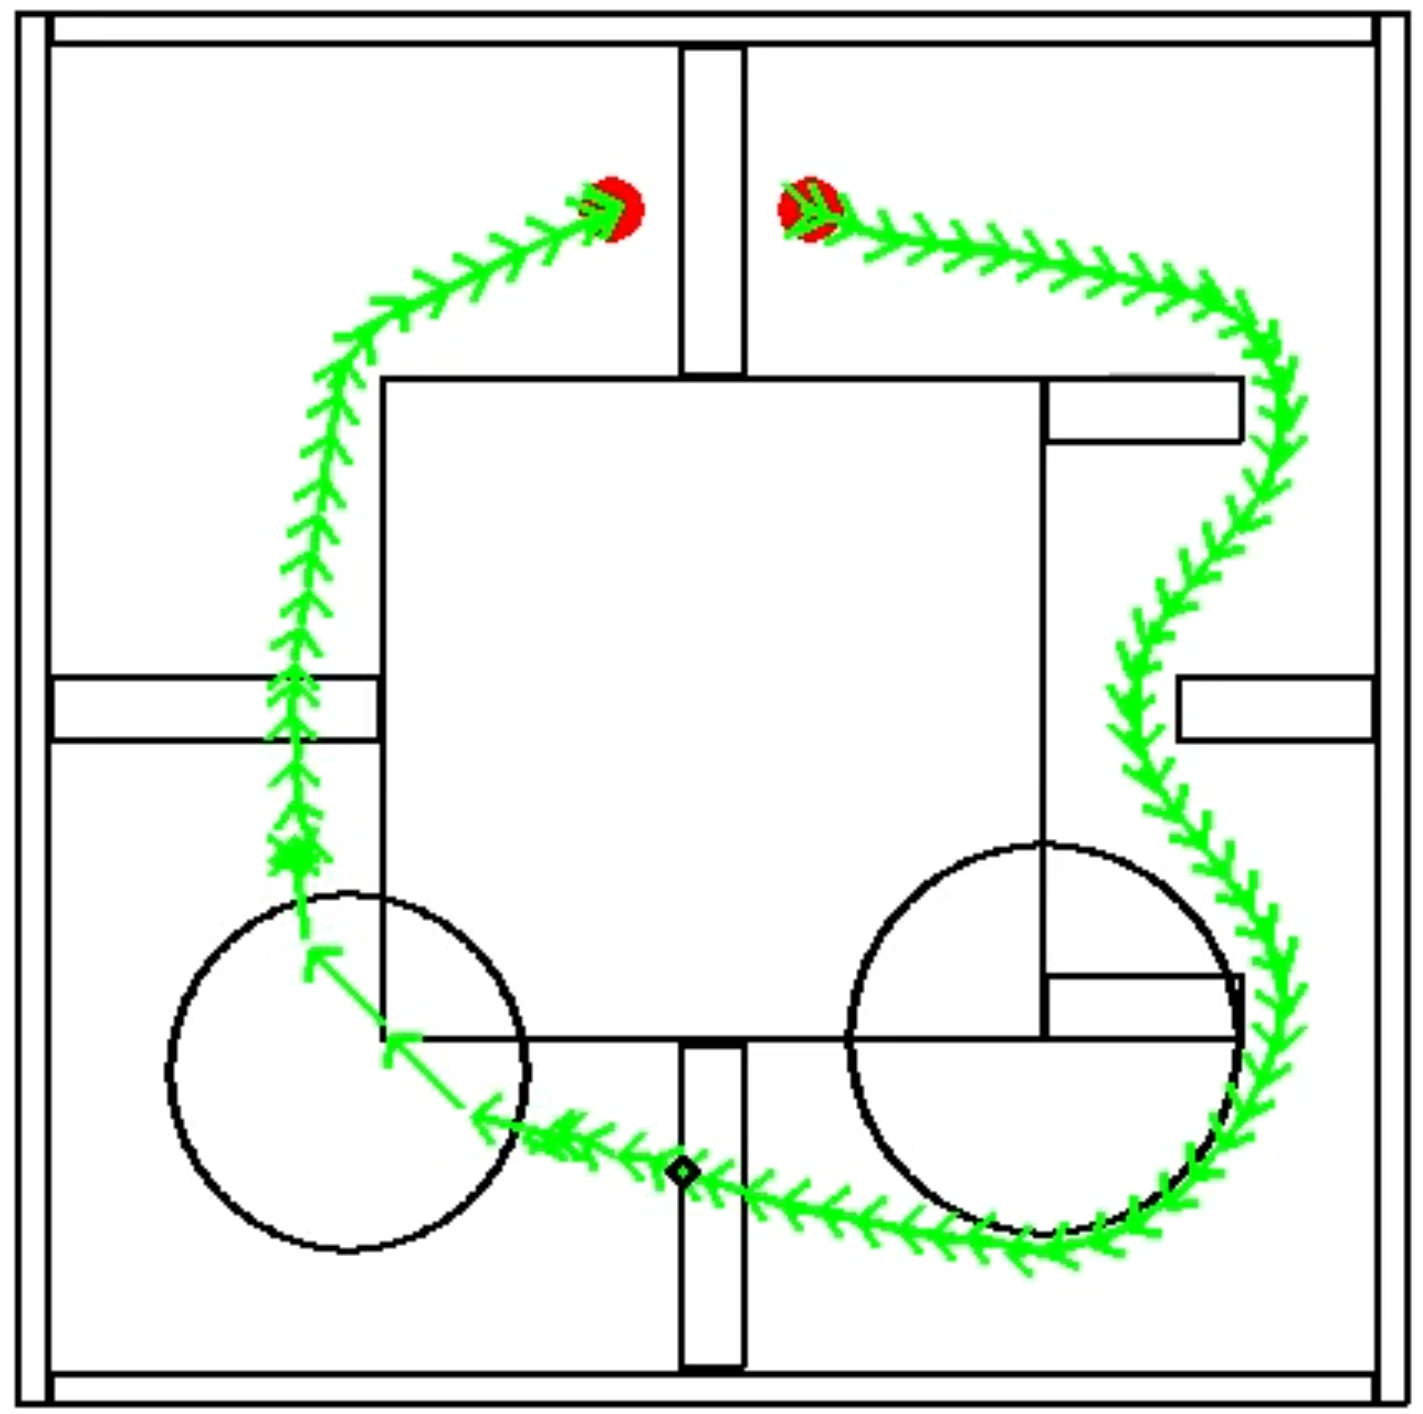
\includegraphics[width=0.8\linewidth]{Figures/07_simulation/basic/08basic.png}
    \end{minipage}%
    \hfill%
    \begin{minipage}[b]{.3\linewidth}
        \centering
        \centering
        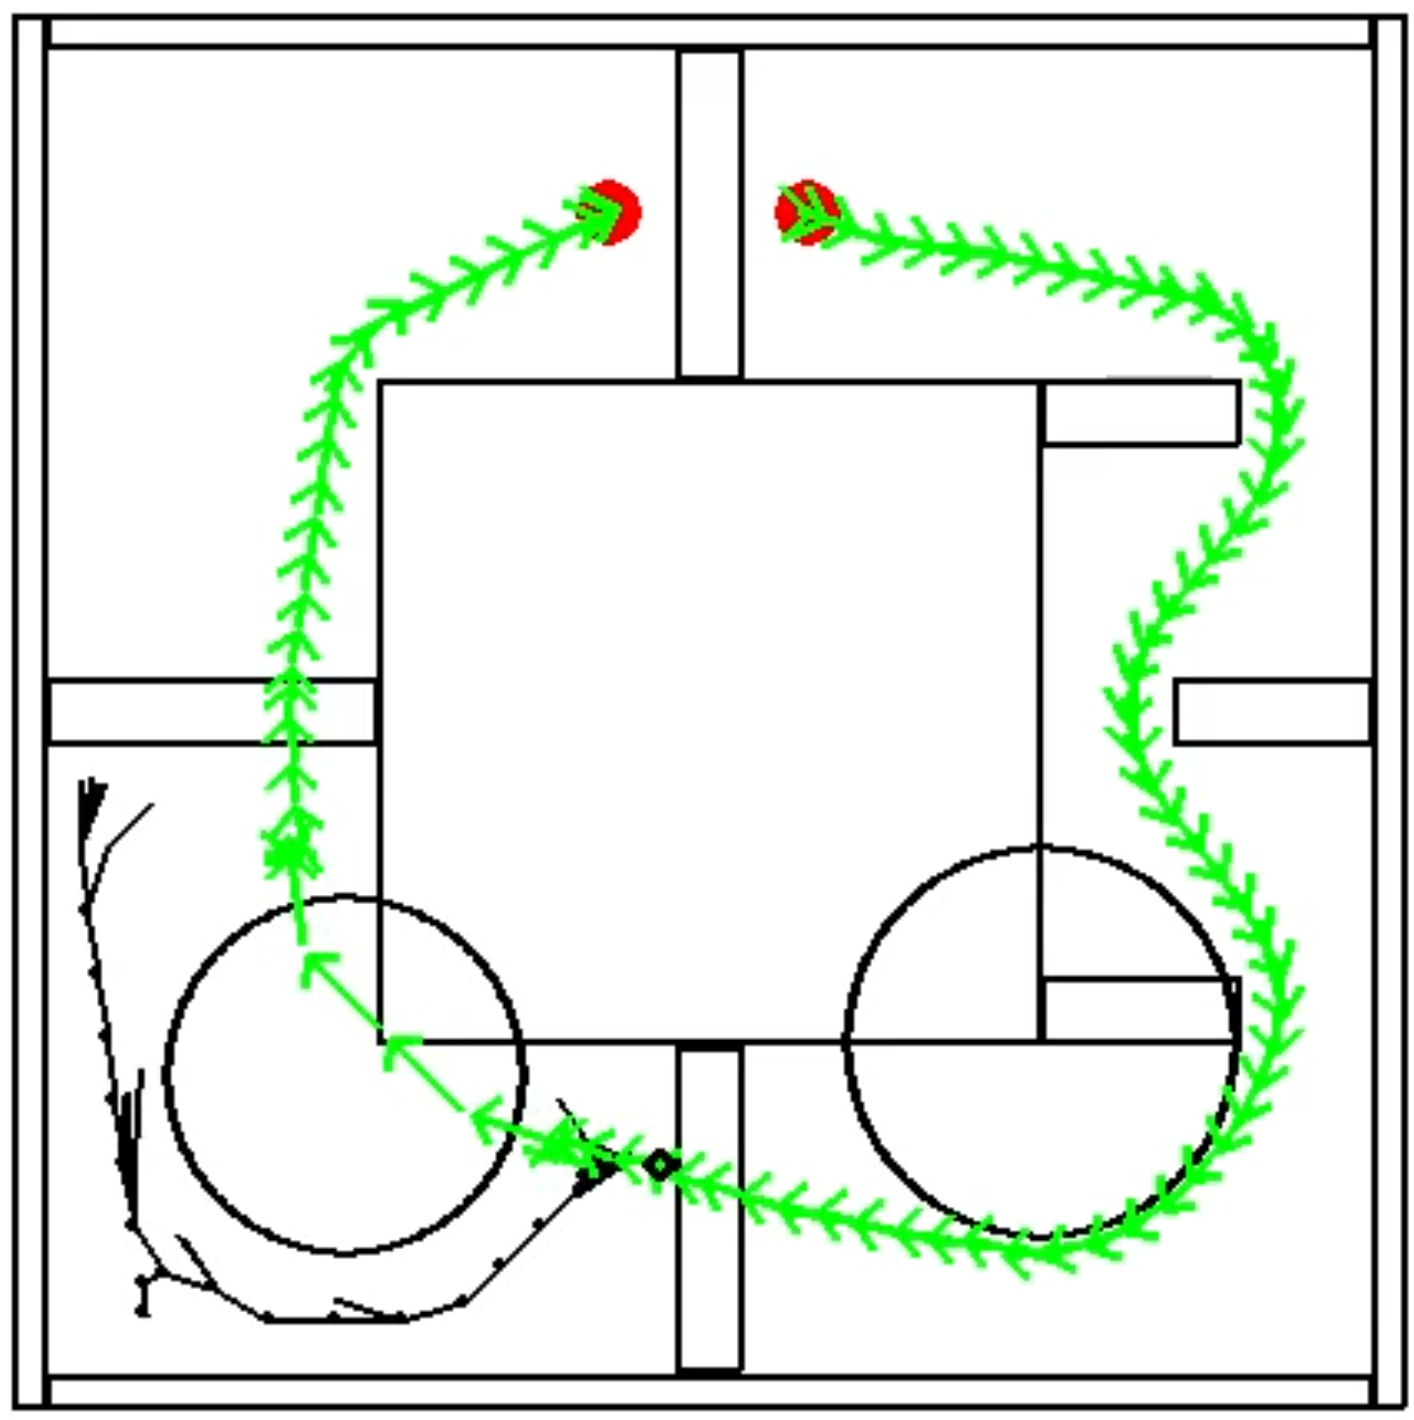
\includegraphics[width=0.8\linewidth]{Figures/07_simulation/basic/09basic.png}
    \end{minipage}%
    \hfill%
    \begin{minipage}[b]{.3\linewidth}
        \centering
        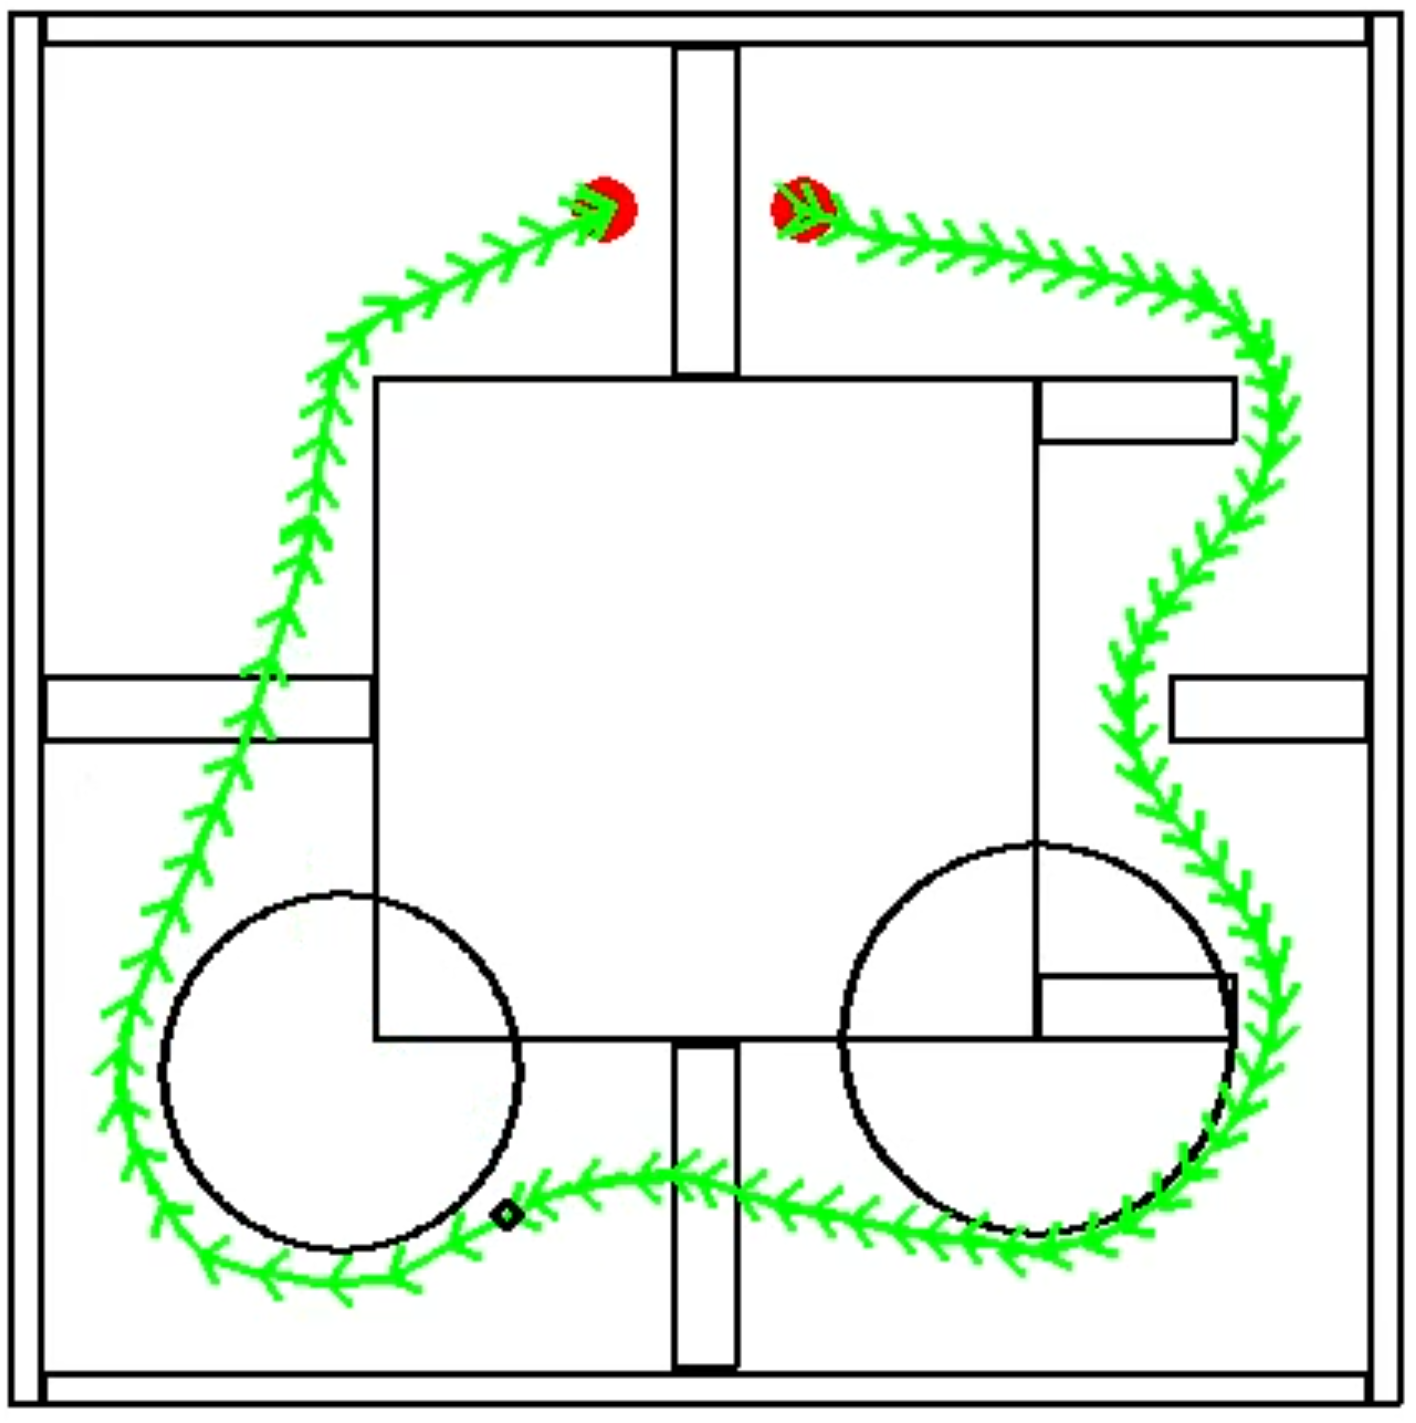
\includegraphics[width=0.8\linewidth]{Figures/07_simulation/basic/10basic.png}
    \end{minipage}\\[-7pt]
    \begin{minipage}[t]{.3\linewidth}
        \caption{Trajectory optimizer gets trapped in an unfeasible local minima (t=46s)}
        \label{fig:basic08}
    \end{minipage}%
    \hfill%
    \begin{minipage}[t]{.3\linewidth}
        \caption{RRT algorithm regrows the critical part of the trajectory (t=47s)}
        \label{fig:basic09}
    \end{minipage}%
    \hfill%
    \begin{minipage}[t]{.3\linewidth}
        \caption{A feasible trajectory is found (t=48s)}
        \label{fig:basic10}
    \end{minipage}%
\end{figure*}


 \begin{figure*}[!htb]
    \centering
    \begin{minipage}[b]{.3\linewidth}
        \centering
        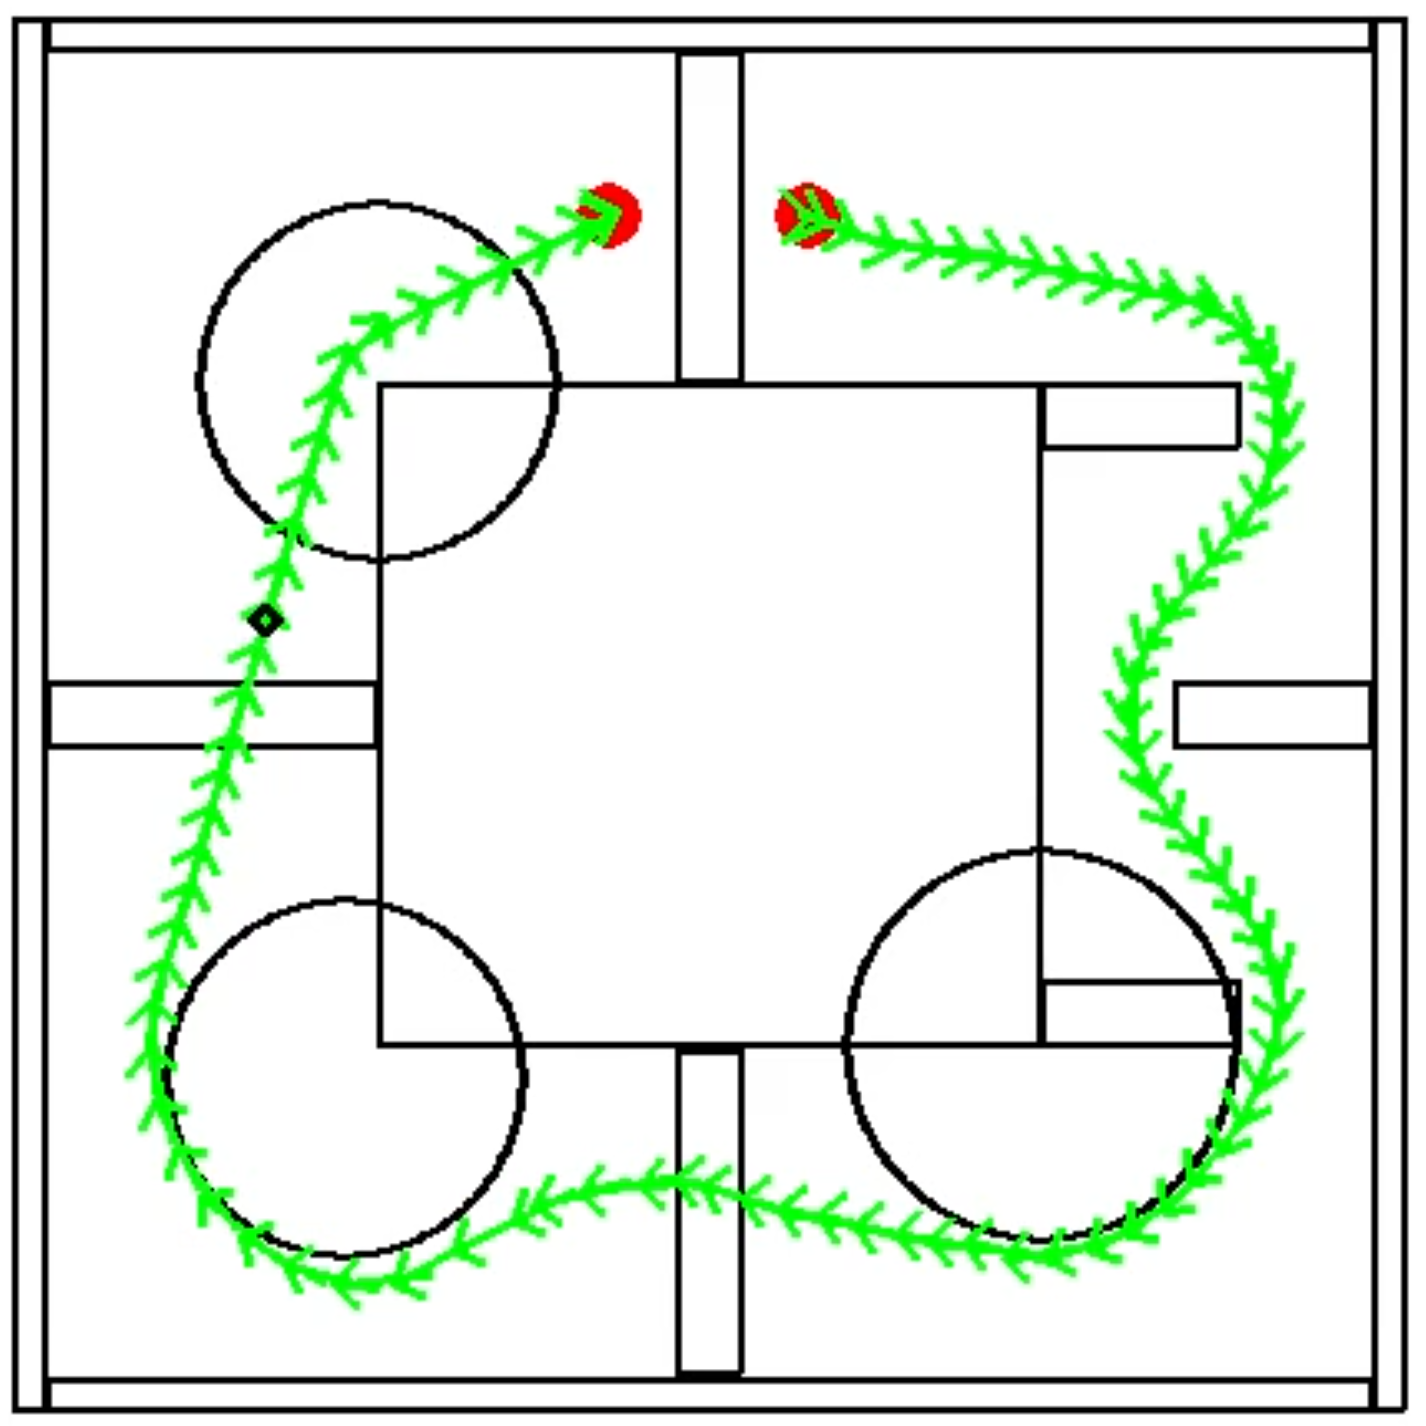
\includegraphics[width=0.8\linewidth]{Figures/07_simulation/basic/12basic.png}
    \end{minipage}%
    \hfill%
    \begin{minipage}[b]{.3\linewidth}
        \centering
        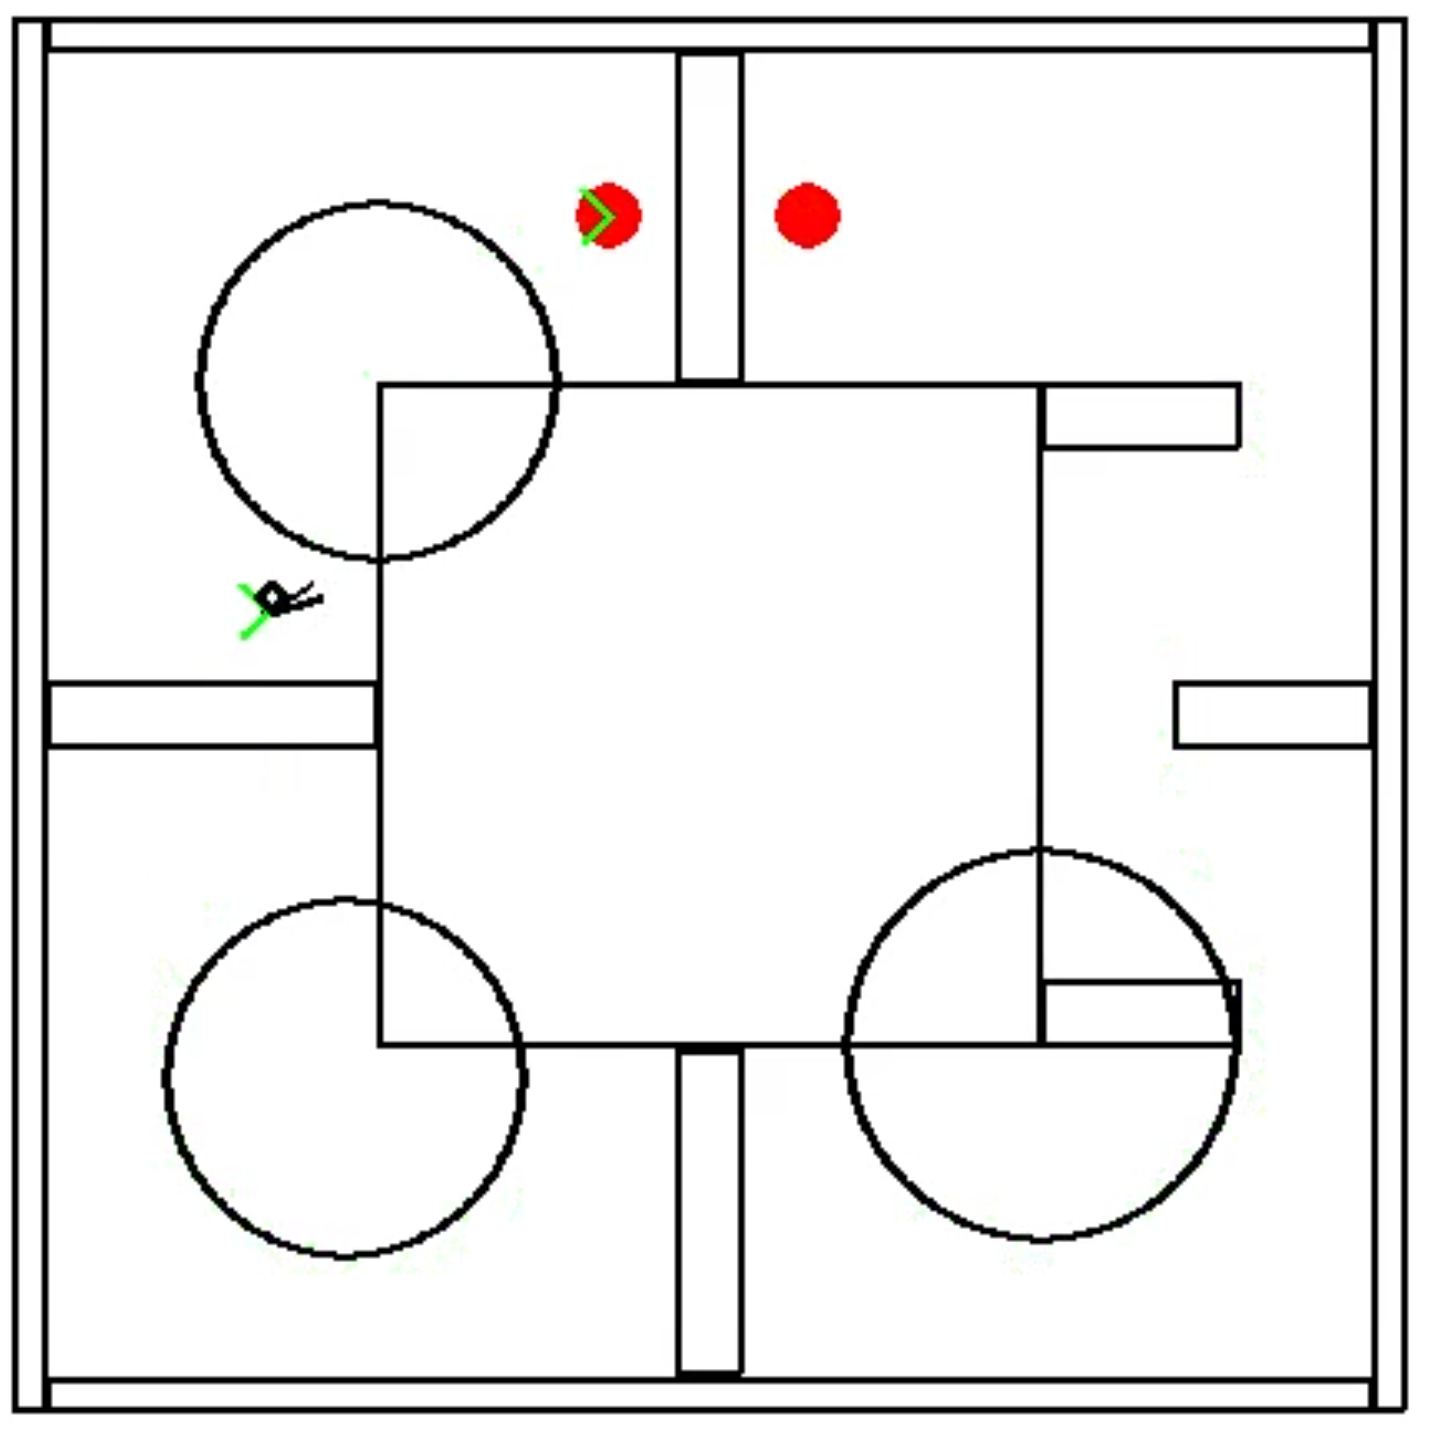
\includegraphics[width=0.8\linewidth]{Figures/07_simulation/basic/13basic.png}
    \end{minipage}%
    \hfill%
    \begin{minipage}[b]{.3\linewidth}
        \centering
        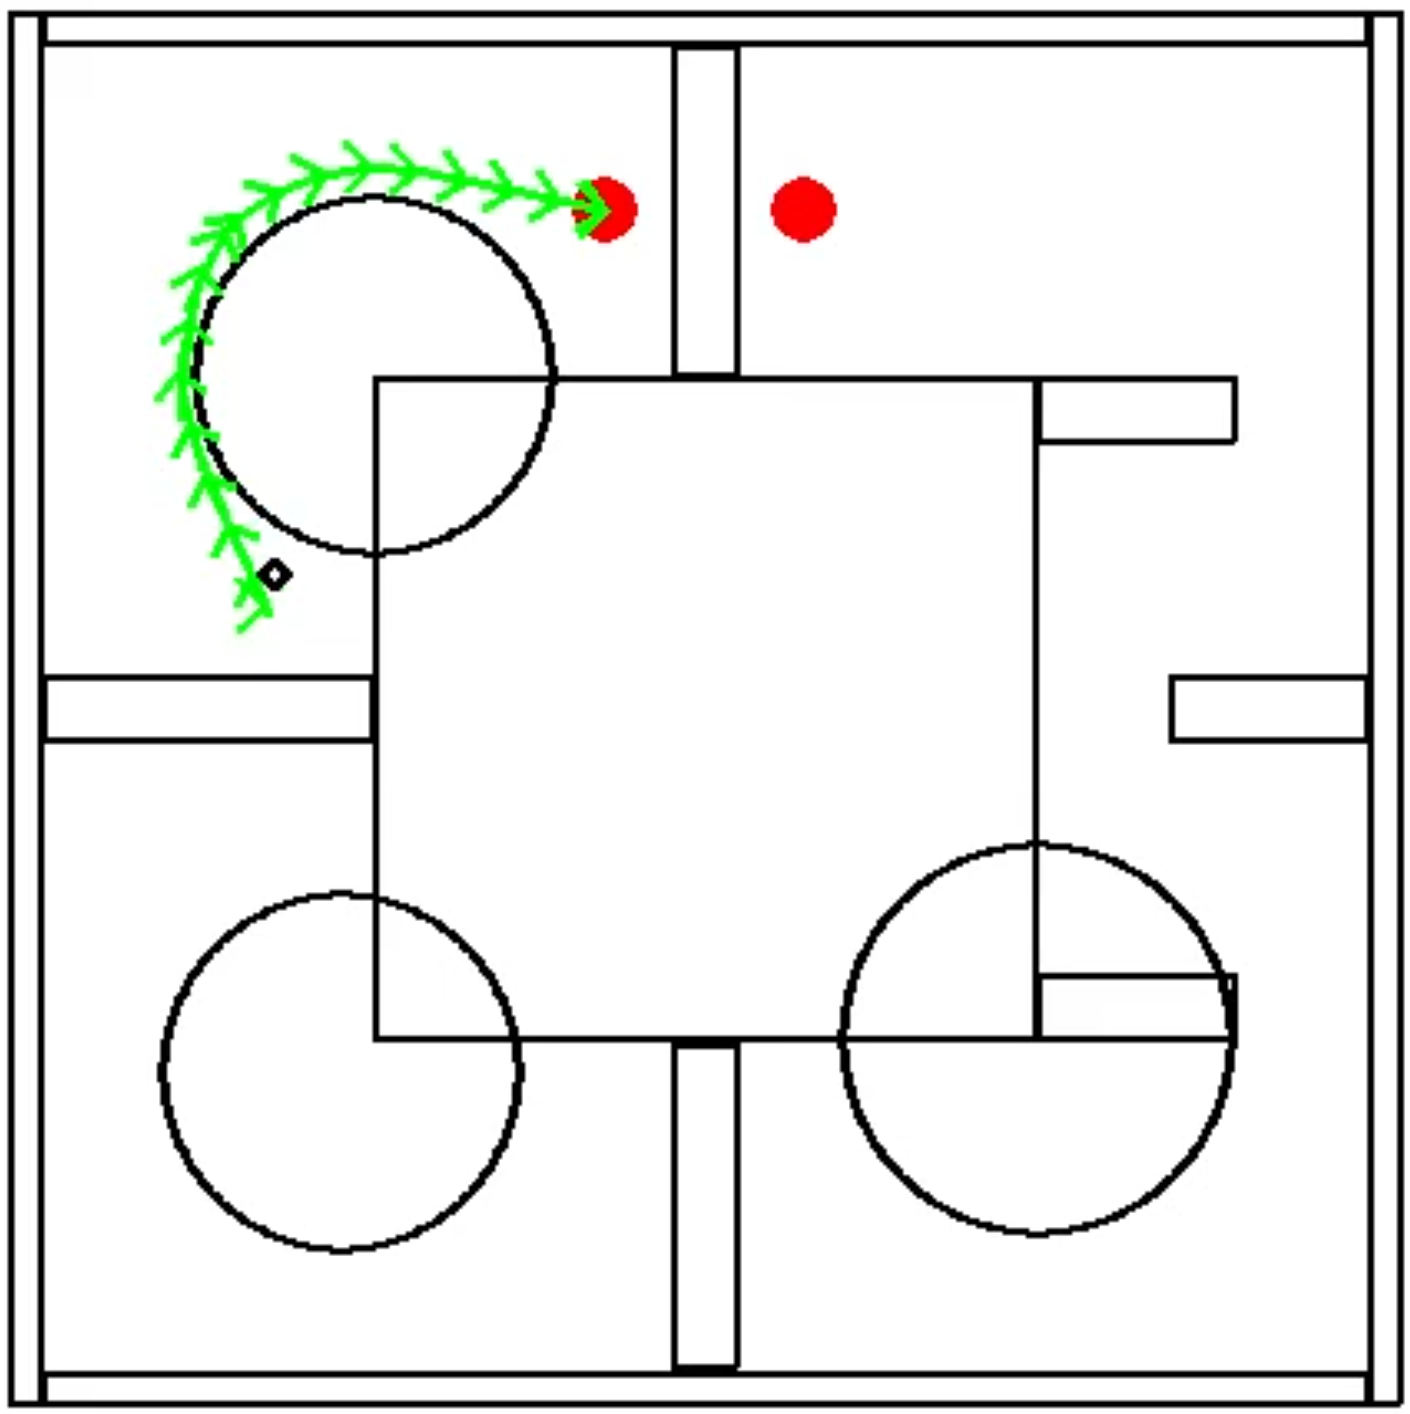
\includegraphics[width=0.8\linewidth]{Figures/07_simulation/basic/14basic.png}
    \end{minipage}\\[-7pt]
    \begin{minipage}[t]{.3\linewidth}
    \caption{Obstacle is detected critically close, trajectory optimizer wouldn't have time to react in real time (t=1m11s)}
    \label{fig:basic12}
    \end{minipage}%
    \hfill%
    \begin{minipage}[t]{.3\linewidth}
    \caption{All references are turned off to prevent the UAV from colliding. Previous trajectory is discarded (t=1m11s)}
    \label{fig:basic13}
    \end{minipage}%
    \hfill%
    \begin{minipage}[t]{.3\linewidth}
    \caption{RRT algorithm regrows a new trajectory from the UAV position to the goal. (t=1m1ss)}
    \label{fig:basic14}
    \end{minipage}%
\end{figure*}


\begin{figure*}[!htb]
    \centering
    \begin{minipage}[b]{.3\linewidth}
        \centering
        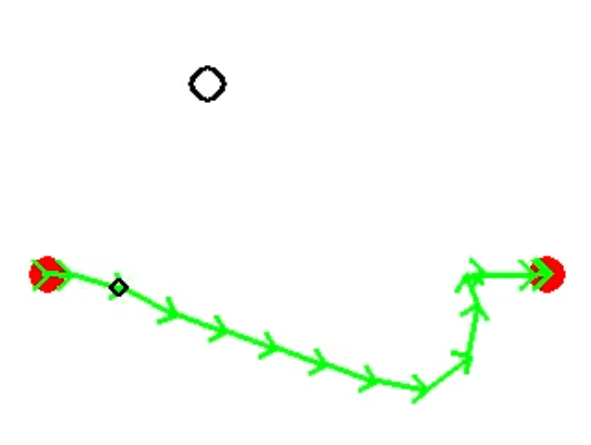
\includegraphics[width=0.8\linewidth]{Figures/07_simulation/nonCoop12/nonCoop11.png}
    \end{minipage}%
    \hfill%
    \begin{minipage}[b]{.3\linewidth}
        \centering
        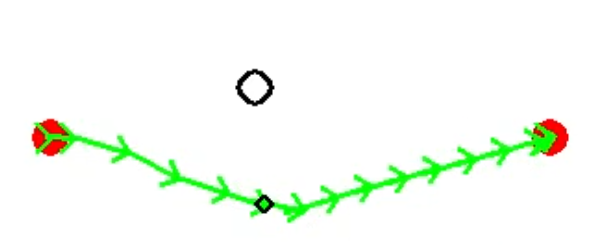
\includegraphics[width=0.8\linewidth]{Figures/07_simulation/nonCoop12/nonCoop12.png}
    \end{minipage}%
    \hfill%
    \begin{minipage}[b]{.3\linewidth}
        \centering
        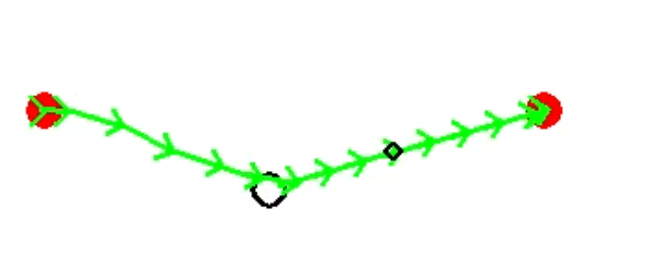
\includegraphics[width=0.8\linewidth]{Figures/07_simulation/nonCoop12/nonCoop13.png}
    \end{minipage}\\[-7pt]
    \begin{minipage}[t]{.3\linewidth}
        \caption{Trajectory while intruder flies to the right}
        \label{nonCoop11}
    \end{minipage}%
    \hfill%
    \begin{minipage}[t]{.3\linewidth}
        \caption{Trajectory changes as intruder changes direction}
        \label{nonCoop12}
    \end{minipage}%
    \hfill%
    \begin{minipage}[t]{.3\linewidth}
        \caption{Intruder is avoided}
        \label{nonCoop13}
    \end{minipage}%
\end{figure*}

 \begin{figure*}[!htb]
    \centering
    \begin{minipage}[b]{.3\linewidth}
        \centering
        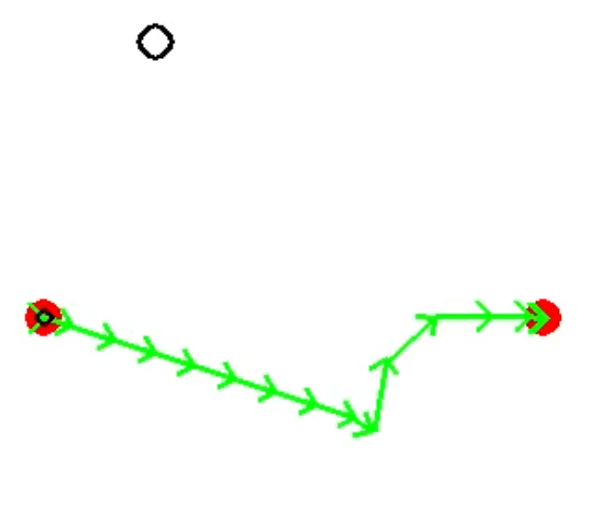
\includegraphics[width=0.8\linewidth]{Figures/07_simulation/nonCoop12/nonCoop21.png}
    \end{minipage}%
    \hfill%
    \begin{minipage}[b]{.3\linewidth}
        \centering
        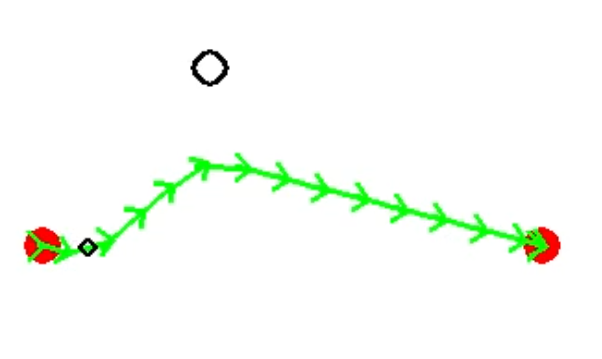
\includegraphics[width=0.8\linewidth]{Figures/07_simulation/nonCoop12/nonCoop22.png}
    \end{minipage}%
    \hfill%
    \begin{minipage}[b]{.3\linewidth}
        \centering
        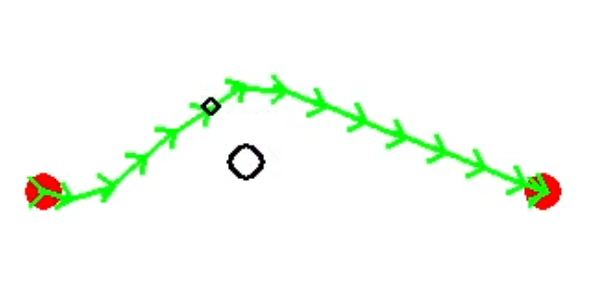
\includegraphics[width=0.8\linewidth]{Figures/07_simulation/nonCoop12/nonCoop23.png}
    \end{minipage}\\[-7pt]
    \begin{minipage}[t]{.3\linewidth}
        \caption{Initially algorithm plans to go below the intruder}
        \label{nonCoop21}
    \end{minipage}%
    \hfill%
    \begin{minipage}[t]{.3\linewidth}
        \caption{Algorithm plans to go above the intruder}
        \label{nonCoop22}
    \end{minipage}%
    \hfill%
    \begin{minipage}[t]{.3\linewidth}
        \caption{Intruder is avoided}
        \label{nonCoop23}
    \end{minipage}%
\end{figure*}

\begin{figure*}[!htb]
    \centering
    \begin{minipage}[b]{.3\linewidth}
        \centering
        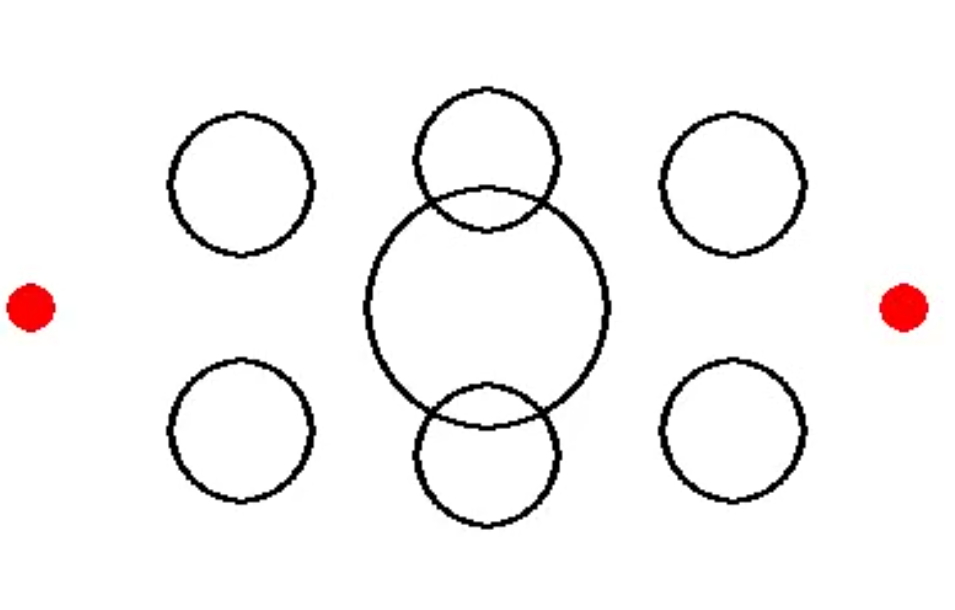
\includegraphics[width=0.9\linewidth]{Figures/07_simulation/lidar/lidar1.png}
    \end{minipage}%
    \hfill%
    \begin{minipage}[b]{.3\linewidth}
        \centering
        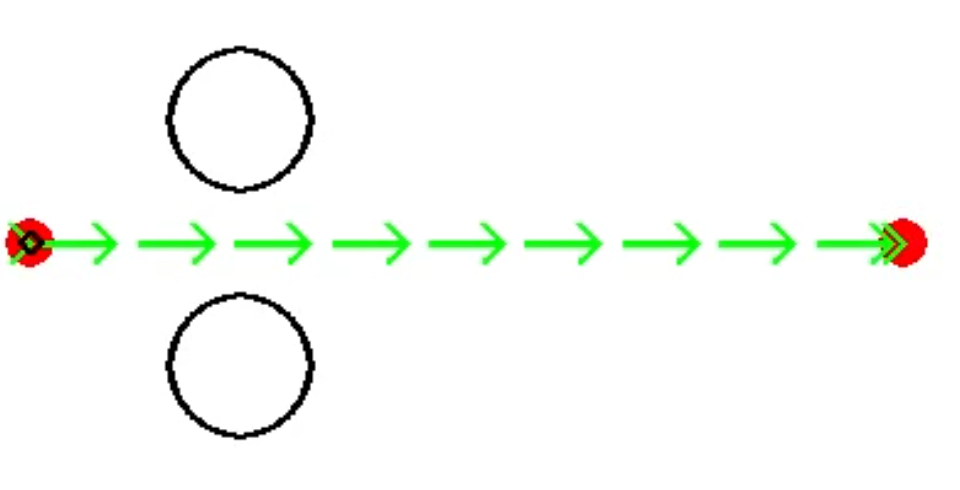
\includegraphics[width=0.9\linewidth]{Figures/07_simulation/lidar/lidar2.png}
    \end{minipage}%
    \hfill%
    \begin{minipage}[b]{.3\linewidth}
        \centering
        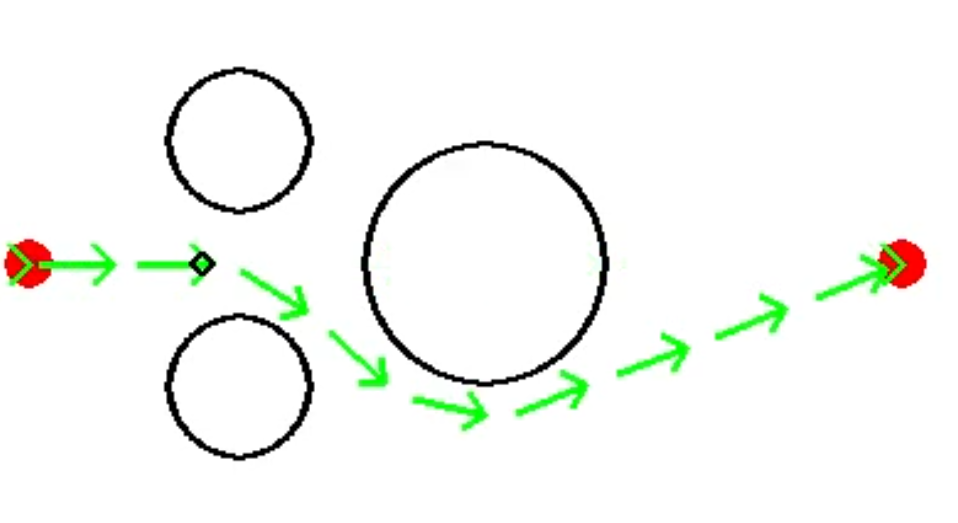
\includegraphics[width=0.9\linewidth]{Figures/07_simulation/lidar/lidar3.png}
    \end{minipage}\\[-7pt]
    \begin{minipage}[t]{.3\linewidth}
    \caption{Complete map}
    \label{fig:lidar1}
    \end{minipage}%
    \hfill%
    \begin{minipage}[t]{.3\linewidth}
    \caption{Initially only two obstacles are visible, none of them interferes with the trajectory}
    \label{fig:lidar2}
    \end{minipage}%
    \hfill%
    \begin{minipage}[t]{.3\linewidth}
    \caption{An obstacle is detected and the trajectory is adjusted.}
    \label{fig:lidar3}
    \end{minipage}%
\end{figure*}

 \begin{figure*}[!htb]
    \centering
    \begin{minipage}[b]{.3\linewidth}
        \centering
        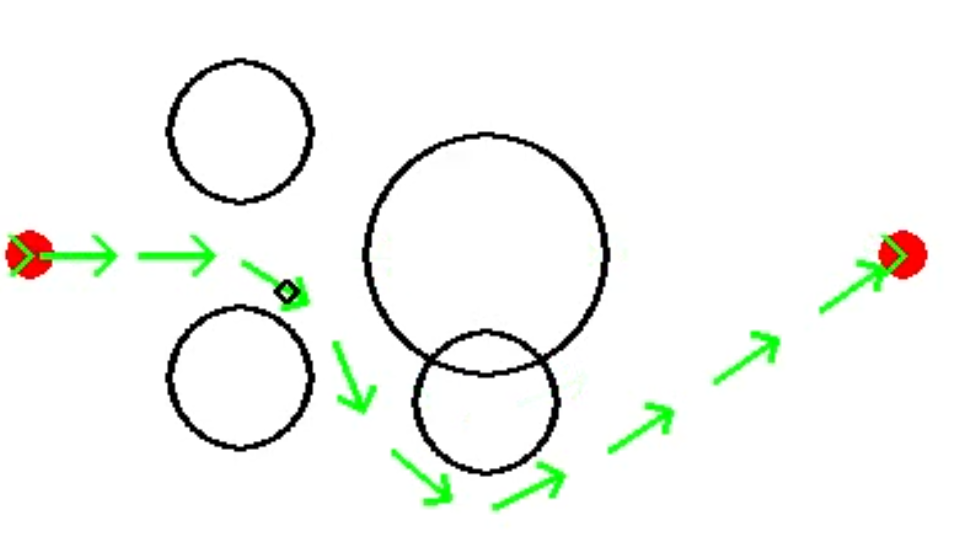
\includegraphics[width=0.9\linewidth]{Figures/07_simulation/lidar/lidar4.png}
    \end{minipage}%
    \hfill%
    \begin{minipage}[b]{.3\linewidth}
        \centering
        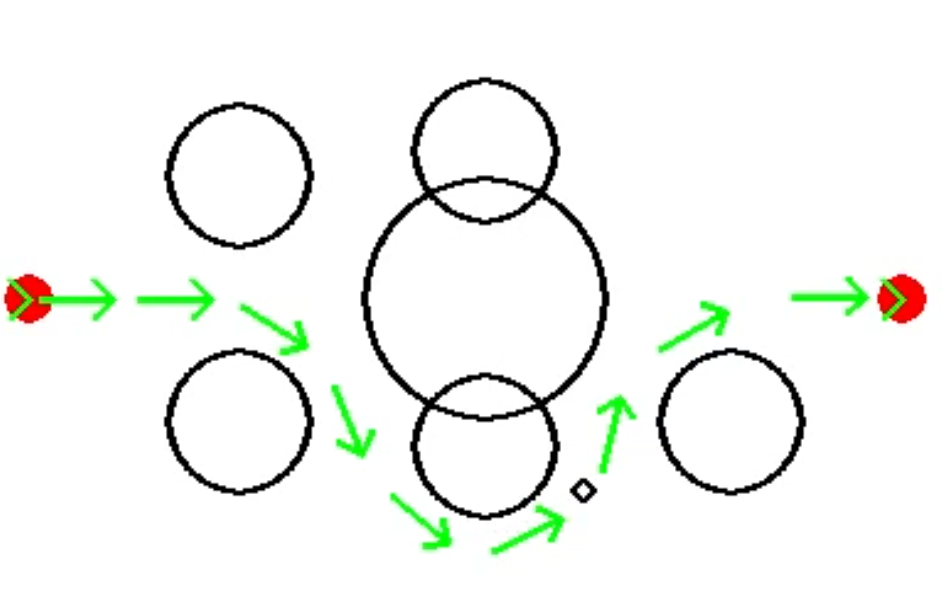
\includegraphics[width=0.9\linewidth]{Figures/07_simulation/lidar/lidar5.png}
    \end{minipage}%
    \hfill%
    \begin{minipage}[b]{.3\linewidth}
        \centering
        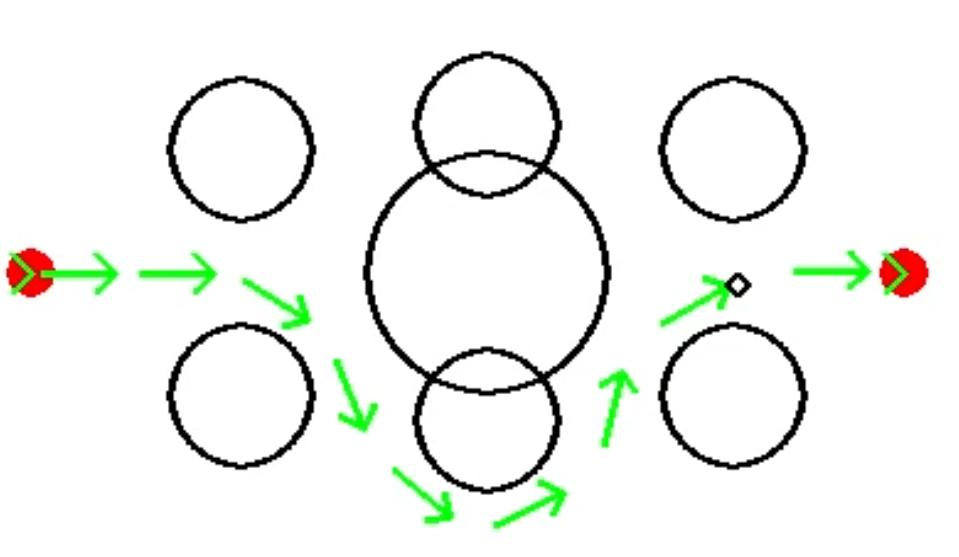
\includegraphics[width=0.9\linewidth]{Figures/07_simulation/lidar/lidar6.png}
    \end{minipage}\\[-7pt]
    \begin{minipage}[t]{.3\linewidth}
    \caption{New obstacle is detected and the trajectory adjusted}
    \label{fig:lidar4}
    \end{minipage}%
    \hfill%
    \begin{minipage}[t]{.3\linewidth}
    \caption{Another obstacle is detected and the trajectory is adjusted}
    \label{fig:lidar5}
    \end{minipage}%
    \hfill%
    \begin{minipage}[t]{.3\linewidth}
    \caption{The final obstacle from the map is detected, it doesn't, however interfere with the trajectory.}
    \label{fig:lidar6}
    \end{minipage}%
\end{figure*}

\begin{figure*}[!htb]
    \centering
    \begin{minipage}[b]{.3\linewidth}
        \centering
        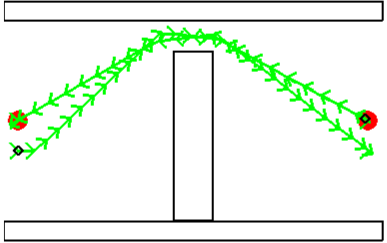
\includegraphics[width=0.6\linewidth]{Figures/07_simulation/basic/twoAir0.png}
    \end{minipage}%
    \hfill%
    \begin{minipage}[b]{.3\linewidth}
        \centering
        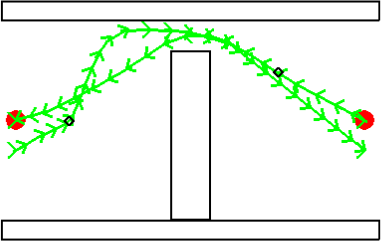
\includegraphics[width=0.6\linewidth]{Figures/07_simulation/basic/twoAir1.png}
    \end{minipage}%
    \hfill%
    \begin{minipage}[b]{.3\linewidth}
        \centering
        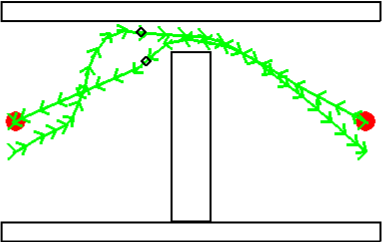
\includegraphics[width = 0.6 \linewidth]{Figures/07_simulation/basic/twoAir2.png}
    \end{minipage}\\[-7pt]
    \begin{minipage}[t]{.3\linewidth}
        \caption{Initial trajectories, computed simultaneously, in collision rout.}
        \label{fig:twoAir0}
    \end{minipage}%
    \hfill%
    \begin{minipage}[t]{.3\linewidth}
        \caption{Collision free trajectories are generated.}
        \label{fig:twoAir1}
    \end{minipage}%
    \hfill%
    \begin{minipage}[t]{.3\linewidth}
        \caption{The aircraft avoid each other (scenario 1).}
        \label{fig:twoAir2}
    \end{minipage}%
\end{figure*}